\chapter{Introduction and Literature Review} % Chapter Title
\label{LR}

\section{The atmosphere}
\label{LR:Atmos}
  % Overarching description of atmosphere
  The atmosphere is made up of gases held to the earth's surface by gravity. 
  These gases undergo transport on all scales, from barbecue smoke being blown about the garden, to smoke plumes from forest fires travelling across the world and depositing in the Antarctic snow.
  They take part in innumerable chemical reactions along the way, largely driven by solar input and interactions with each other.
  Many gases are emitted into the atmosphere by soil, trees, factories, cars, seas and oceans.
  They are also deposited back to the surface both directly and in rainfall.
  
  % Air
  The atmosphere is made up of nitrogen (N$_2$: $\sim 78\%$), oxygen (O$_2$: 
  $\sim 21\%$), and argon (Ar: $\sim 1\%$), along with water (H$_2$O) and 
  \textit{trace gases} (those that make up less than 1\% of the atmosphere).
  Atmospheric H$_2$O content can be as high as $4\%$ depending on local 
  conditions.
  Beyond these major constituents the atmosphere has a vast number of trace 
  gases, including carbon dioxide (CO$_2$: $\sim 0.4\%$), ozone (O$_3$: 
  $.000001\%$ to $0.001\%$), and methane (CH$_4$: $\sim 0.00018\%$) 
  \parencite[][Ch. 2]{NOAAch4, BrasseurJacob2017}.
  Trace gases in the atmosphere can have a large impact on conditions for life on earth.
  They combine, break apart, and react with each other affecting all surface ecosystems upon which life depends.
  
  One important trace gas is ozone (O$_3$), which affects climate, human health, and ecosystem productivity.
  The ozone budget (production, loss, and transport) is relatively uncertain 
  over Australia.
  This thesis focuses on ozone in the troposphere over Australia and sites in 
  the nearby Southern Ocean.
  It also estimates emissions of isoprene, one of the important precursors to tropospheric ozone production.
  This chapter provides background on the structure and composition of the 
  atmosphere and introduces the key atmospheric species examined in this 
  thesis, as well as relevant techniques used to measure and model chemistry in 
  the atmosphere.
  %Ozone is discussed in more detail in Section \ref{LR:O3}.
  %Another important atmospheric class of compounds examined in this thesis is called volatile organic compounds (VOCs) and is introduced in Section \ref{LR:VOCs}.
  
  
  \subsection{Structure}
  \label{LR:Atmos:Struct}
    
    Most of the atmosphere ($\sim 85\%$) is within 10~km of the earth's surface.
    This is due to gravity, which causes air pressure to decrease logarithmically with altitude.
    Any entity is subjected to the weight of the air above it, and the 
    structure of the atmosphere is driven by this pressure.
    
    The atmosphere extends above the earth's surface to the edges of space. 
    This is split into various layers, defined by the \textit{lapse rate}: the decrease in temperature (\textit{T}) with increasing altitude (\textit{z}), or $\frac{-\textrm{d}T}{\textrm{d}z}$.
    Figure \ref{LR:Atmos:Struct:Fig_atmos_layers} shows the pressure and temperature profiles against altitude through the atmosphere.
    The first layer is the troposphere, which extends to roughly 10~km and is characterised by positive lapse rate (or decreasing temperature with altitude).
    At the top of the troposphere (the tropopause) the temperature stops decreasing, and then the stratosphere is defined by a negative lapse rate.
    This is due to ultraviolet radiation being absorbed by ozone, and leads to a very vertically stable environment.
    
    \begin{figure}
      \includegraphics[width=\textwidth]{Figures/Atmos_Temp_Press.jpg}
      \caption{%
        Pressure (red) logarithmically decreasing, shown with percentage of atmosphere below at several points.
        Temperature (green) changes throughout the atmosphere.
        Figure modified from \url{https://climate.ncsu.edu/edu/Structure}.
      }
      \label{LR:Atmos:Struct:Fig_atmos_layers}
    \end{figure}
    
    
    
    % Boundary layer
    In addition to these atmospheric layers, the troposphere can be subset into the \textit{boundary layer} and the \textit{free troposphere}.
    The \textit{boundary layer} is the lowest layer and involves increased atmospheric mixing due to ground heating and friction effects.
    It generally extends from the surface up to 200~m - 1000~m, above which the ground effects have fewer direct impacts.
    The \textit{free troposphere} is the remainder of the troposphere, where 
    trace gas concentrations are more affected by transport and chemistry.
    Transported trace gases (and particulates) can come from the stratosphere 
    or local to global scale winds and jet streams.
    
    
  % Chemistry
  \subsection{Composition and chemistry}
  \label{LR:Atmos:Chem}
        
    There are myriad trace gases in the atmosphere, emitted by plants, animals, 
    earth, and water. 
    These gases react with one another and over time they either deposit back 
    onto the earth or form more stable compounds such as carbon dioxide 
    (CO$_2$).
    Oxidation and photolysis (the process of being broken apart by photons) are the two main processes whereby compounds are broken down in the atmosphere.
    Products formed in these reactions are sometimes called child products.
    
    % Oxidation and Radicals
    %\subsubsection{Hydroxyl radicals}
    %\label{LR:Atmos:Chem:radicals}
    Hydroxyl radicals (OH$\dot{}$) and hydrogen dioxide (HO$_2$) concentrations 
    largely determine the oxidative capacity of the atmosphere.
    The OH radical drives many processes in the atmosphere, especially during 
    the day when it is produced by the photolysis of ozone \parencite{Atkinson2000}.
    OH is a key species that reacts with nearly all the organic compounds in the troposphere, with only a few exceptions \parencite{Atkinson2000}.
    %The exceptions are chlorofluorocarbons (CFCs), and Halons not containing H atoms \parencite{Atkinson2000}.
    Over land, isoprene (C$_5$H$_8$) and monoterpenes (C$_{10}$H$_{16}$) account for 50\% and 30\% of the OH reactivity respectively \parencite{Fuentes2000}.
    
    Since radicals are involved in all oxidative chemistry in the atmosphere it 
    is important for models to accurately represent them 
    \parencite[e.g.,][]{Travis2016}.
    This is difficult as they are coupled with so many other species and measurements of OH are not readily available on a global scale.
    In the late 1990s it was thought that OH radicals were formed exclusively 
    from photolysis of O$_3$, HONO, HCHO, and other carbonyls (R$_2$C=O) 
    \parencite{Atkinson2000}.
    It has been shown since that OH is recycled in various processes.
    For example isoprene (C$_5$H$_8$) was thought to be a sink of OH until it 
    was shown by \textcite{Paulot2009b} that the radicals are recycled.
    This recycling process is discussed in more detail in section \ref{LR:VOCs:IsopCascade}.
    
    Ozone is an important precursor to OH, as excited oxygen atoms (O(${}^1$D)) 
    are created through its photolysis, which then go on to react with water to 
    form OH, as shown in reaction sequence \ref{LR:Atmos:Chem:eqn_O3toOH} 
    \parencite{Atkinson2000, AtkinsonArey2003}:
    \begin{equation}
      \begin{aligned}
        O_3+hv            & \to  O_2 + O({}^1D)   && (\lambda \le 350 \text{nm}) \\%
        O({}^1D)+M        & \to  O({}^3P) + M     && (M=N_2, O_2)               \\%
        O({}^3P)+O_2 + M  & \to  O_3 + M          &&                           \\%
        O({}^1D)+H_2O     & \to  2OH              &&                            \\%
      \end{aligned}
      \label{LR:Atmos:Chem:eqn_O3toOH}
    \end{equation}
    where $hv$ represents radiation and M is an inert molecule.
    This shows that some of the O$({}^1D)$ recycles back to ozone, while some 
    forms OH.
    %\textcite{AtkinsonArey2003} discuss the relative rates of these reactions.
      
\section{Ozone}
\label{LR:O3}
  
  Ozone (O$_3$) is an important greenhouse gas and oxidant.
  It is mostly located in the stratosphere and prevents much of the shorter wavelength solar radiation from reaching the earth's surface.
  Ozone in the troposphere is less beneficial, leading to health issues, 
  radiative forcing, and crop death \parencite{Stevenson2013}.
  Understanding and accurately portraying ozone concentrations in the troposphere is important to allow accurate predictions of future climate.
  This will become even more important as climate change alters the atmosphere 
  \parencite{Hegglin2009}.
  %Projections of future climate change include changes to several atmospheric 
  %parameters such as vertical mixing rates, the ultra violet index, and ozone 
  %radiative forcing \parencite{Hegglin2009}.
  
  \subsection{Stratospheric ozone}
  
    %Structure of ozone layer chapman eqn etc.
    In the stratosphere, ozone production is driven by the Chapman mechanism, as high energy radiation (with wavelengths $\lambda<242$~nm) photolyses the molecular oxygen (O$_2$) in the atmosphere \parencite[][Chapter 3, section 2]{BrasseurJacob2017}.
    The Chapman mechanism involves several reactions that lead to rough equilibrium of O, O$_2$, O$_3$ and pressure, as follows:
    \begin{equation}
      \begin{aligned}
        \text{O}_2 + hv              & \to \text{O}+\text{O}     && \lambda < 242 \text{nm} \\
        \text{O}+\text{O}_2+\text{M} & \to \text{O}_3+\text{M}   &&    \\
        \text{O}_3 + hv              & \to \text{O}+\text{O}_2   && \lambda < 1180 \text{nm} \\
        \text{O} + \text{O}_3        & \to \text{O}_2+\text{O}_2 &&       \\
      \end{aligned}
      \label{LR:O3:eqn_Chapman}
    \end{equation}
    The high energy photons ($\lambda < 242$~nm) are present from the top of the atmosphere but are mostly removed before reaching the troposphere as their energy is used to split the O$_2$ molecules.
    The lifetime of O against loss by O$_2$ is less than a second in the troposphere, and produced O$_3$ quickly returns to O and O$_2$, as low energy ($\lambda < 1180$~nm) photons and M are abundant.
    The reduced light penetration towards the surface, in addition to the logarithmic increase in atmospheric pressure (which affects M abundance) drives the vertical profile of ozone into what is called the \textit{ozone layer}.
    This is a layer of relative ozone abundance within the stratosphere.
    %The Chapman mechanism requires radiation so only takes place during the 
    %daytime.
    %During the night this process slows to a halt, and the ozone 
    %concentrations remain stable unless pollution intrudes \parencite[Chapter 
    %10]{Jacob_1999_book}.
  
    
    % Measurements
    Satellite based measurements of ozone were instrumental in identifying the 
    ozone hole.
    Since the Montreal Protocol on Substances that Deplete the Ozone Layer was 
    established in August 1987, and ratified in August 1989, new satellites and 
    measurement stations were set up to monitor ozone in the stratosphere.
    Detecting ozone from the surface up to the top of the stratosphere requires techniques such as remote sensing and ozonesonde releases.
    Ozonesondes are weather balloons (with attached ozone detectors) that detect ozone concentrations up to the mid stratosphere ($\sim 30$~km), providing a vertical profile over a single location.
    %Since 1986, Lauder, New Zealand (45$^{\circ}$S, 170$^{\circ}$E) has released ozonesondes allowing a multi-decadal analysis of ozone concentrations over the city \parencite{Brinksma2002}.
    Ozonesondes have been released periodically for decades over some cities, allowing long term ozone concentration profile analysis \parencite[e.g.,][]{Brinksma2002}.
    %Kerguelan Island (49.2$^{\circ}$S, 70.1$^{\circ}$E), also has a record of ozonesonde profiles, which are directly in the path of biomass burning smoke plumes transported off shore from Africa \parencite{Baray2012}.
    %SHADOZ is the southern hemispheric additional ozone project, which have released sondes from 15 sites at different times \url{http://tropo.gsfc.nasa.gov/shadoz/}.
    A small network of ozonesonde release sites (including Davis, Macquarie Island, and Melbourne) is available from the world ozone and ultraviolet radiation data centre \url{http://woudc.org/data/explore.php} and is used in Chapter \ref{Ozone} to examine stratospheric impacts on tropospheric ozone (see Section \ref{Model:datasets:ozonesondes} for more info on these ozonesondes).
  
  \subsection{Tropospheric ozone}
    
    Ozone in the lower atmosphere is a serious hazard that causes health problems \parencite{Hsieh2013}, causes billions of dollars of damage to agricultural crops \parencite{Avnery2011, Yue2017}, and increases the rate of climate warming \parencite{IPCC_2013_chap8}.
    Around 5 to 20 percent of all air pollution related deaths are due to ozone \parencite{Monks2015}, which translates to roughly 800 thousand deaths per year \parencite{Lelieveld2013}.
    In the short term, ozone concentrations of $\sim$50-60~ppbv over eight hours or $\sim$80~ppbv over one hour are agreed to constitute a human health hazard \parencite{Ayers2006, Lelieveld2009}. 
    Long term exposure causes problems with crop loss and ecosystem damage \parencite{Emberson2003}, and concentrations may get worse in the future \parencite{Lelieveld2009, Stevenson2013}.
    For example, future tropospheric ozone enhancements are projected to drive 
    reductions in global crop yields equivalent to losses of up to 
    \$USD$_{2000}$ 35 billion (US dollars in the year 2000) per year by 2030 
    \parencite{Avnery2011}, along with detrimental health outcomes equivalent 
    to $\sim$\$USD$_{2000}$11.8 billion per year by 2050 \parencite{Selin2009}.
    Recently \textcite{Yue2017} showed that the net effect of near-surface ozone is an approximately $14\%$ decrease in net primary productivity in China.
    They also state that in order to wind back most of this productivity decrease, drastic measures are required. %(by $\sim 70\%$ before 2030)
    
    Figure \ref{LR:O3:fig_YoungOzoneSummary}, reproduced from \textcite{Young2018}, shows a summary of the major processes and emissions affecting tropospheric ozone.
    This thesis focuses on improving the highly uncertain natural emissions of 
    non-methane volatile organic compounds (NMVOCs) from Australia, and 
    estimating how much ozone is transported down from the stratosphere.
    
    \begin{figure}
      \includegraphics[width=\textwidth]{Figures/Young2018_Figure1.png}
      \caption{%
        Tropospheric ozone processes, Figure 1 in \textcite{Young2018}.
        DOI: https://doi.org/10.1525/elementa.265.f1
      }
      \label{LR:O3:fig_YoungOzoneSummary}
    \end{figure}
  
    %What drives ozone in the troposphere? 
    Generally there are two main drivers of tropospheric ozone concentrations: 
    transport from the stratosphere and chemical production due to emissions of 
    precursors. 
    % Loss pathways
    Tropospheric ozone is lost via chemical destruction and dry deposition, 
    estimated to be $4700\pm700$ Tg yr$^{-1}$ and $1000\pm200$ Tg yr$^{-1}$, 
    respectively \parencite{Stevenson2006, Young2018}.
    The main loss channel is through photolysis and collisions, and leads to OH 
    production (equation \ref{LR:Atmos:Chem:eqn_O3toOH}).
  
  \subsubsection{Stratosphere to troposphere transport}
    \label{LR:O3:STT}
    %% STT
    Historically, ozone transported down from the stratosphere was thought to contribute 10-40~ppb to tropospheric ozone levels, making up 50\% of tropospheric concentrations \parencite{Atkinson2000, Stohl2003}.
    The proportion was revised down to around 10\% over the years as measurement and modelling campaigns improved our understanding of global scale transport, mixing, and chemistry \parencite{Guenther2006, Monks2015}.
    Intrusions of stratospheric air into the troposphere are often called Stratosphere to Troposphere Transport (STT) events.
    Although most tropospheric ozone comes from production, STT enhancements of 
    ozone are measurable and can be regionally important 
    \parencite[eg.,][]{Jacobson2000, Lelieveld2009, Kuang2017}.
    Additionally, upper tropospheric ozone can be transported long distances 
    \parencite{Cooper2004}, affecting measurements far downwind of where 
    stratospheric mixing may be taking place.
    An analysis of the Atmospheric Chemistry and Climate Model Inter-comparison Project (ACCMIP) simulations showed STT enhances tropospheric ozone by $540\pm140$~Tg yr$^{-1}$ \parencite{Young2013}, equivalent to $\sim$11\% of the tropospheric ozone column \parencite{Monks2015}.
    
    
    Ozone transported to the troposphere from the stratosphere can occur through diffusion (relatively slowly) or direct mixing (as STT).
    STT often occur as tongues of stratospheric air that descend into the troposphere before becoming detached.
    These can be due to low pressure systems and jet streams \parencite{Sprenger2003}.
    It is possible to model this process and estimate how much ozone is being 
    transported by STT \parencite[e.g.,][]{Young2013, Ojha2016}.
    Model based estimates require validation against actual measurements, such as those from ozonesondes or satellites.
    %Hegglin, M. I., and T. G. Shepherd (2009), Large climate-induced changes in ultraviolet index and stratosphere-to-troposphere ozone flux, Nature Geosci, 2(10), 687 \selectlanguage{english}691, doi:10.1038/NGEO604.
    It has been estimated that climate change will lead to increased STT 
    through acceleration of the Brewer Dobson circulation 
    \parencite{Hegglin2009}, a large scale transport system that affects the 
    structure and composition of the atmosphere, and meteorology, in the 
    tropics.
    \textcite{Hegglin2009} estimated that ozone transport would increase by 
    23\% globally by 2095 (relative to 1965), $\sim 30$\tgpyr ~in the southern 
    hemisphere and $\sim 121$\tgpyr ~in the northern hemisphere.
    
    %%One way to analyse ozone and its driving processes is to examine its inter-annual variability (IAV).
    %%IAV is the standard deviation of ozone anomalies from the monthly mean.
    STT mostly impacts the upper troposphere, although some areas are impacted 
    down to the surface.
    Over both ocean and land STT can lead to seasonal enhancements of upper and 
    lower tropospheric ozone concentrations 
    \parencite{Lin2015, Liu2017, Kuang2017}.
    A confounding factor is that stratospheric based ozone enhancement can be 
    transported horizontally, and is not confined to the area where intrusion 
    into the troposphere occured.
    %Near-surface ozone concentrations also depend on the local topography, 
    %weather systems, and trace gases emitted and transported into the region.
    %Emissions or pollution plumes transported internationally can affect ozone 
    %concentrations, and the 
    Understanding of STT needs to be improved to allow source attribution of 
    the causes of local ozone enhancements \parencite{Lin2015}.
    %\textcite{Liu2017} show that ozone transported from the stratosphere plays a major role in the upper troposphere, especially over the southern Indian ocean during austral winter.
    %\textcite{Kuang2017} found a measurable impact of STT ozone enhancement in the south east US using several different instruments. 
    %\textcite{Liu2017} examined modelled tropospheric ozone sensitivity to various meteorological parameters.
    %They showed that ozone at 430~hPa (roughly 6~km altitude) is mostly stratospheric in September over 20$^{\circ}$S to 60$^{\circ}$S at all longitudes.
    %In the USA, tropospheric ozone is sensitive to emissions from South America (0--20$^{\circ}$S, 72.5--37.5$^{\circ}$W), southern Africa (5--10$^{\circ}$S, 12-38$^{\circ}$E), and South to South east Asia (70-125$^{\circ}$E, 10$^{\circ}$S--40$^{\circ}$N).
    %In the US recent work by \textcite{Lin2015} suggests that intrusions during spring are increasing surface ozone levels.
    %They recommend improvements to understanding of the frequency and cause of STT are needed effectively implement air quality standards.
    
    % Uncertainties?
    
  % UP TO HERE readthrough
  \subsubsection{Chemical production}
    
    
    Tropospheric ozone concentrations are enhanced by ozone precursor 
    emissions; including NO, NO$_2$, CO, and VOCs such as isoprene 
    \parencite{Atkinson2000, Young2013, Marvin2017}.
    Ozone predictions are uncertain and changing climate affects transport, 
    deposition, destruction, and natural precursor emissions.
    All of these processes are tightly coupled and difficult to accurately 
    model, as they depend on uncertain assumptions such as CO$_2$ dependency 
    \parencite{Young2013}.
    Despite significant advances over the prior decades, there remain large 
    uncertainties about ozone precursors in the troposphere 
    \parencite{Mazzuca2016}.
    Tropospheric ozone is regulated by NO and NO$_2$ concentrations, which form 
    an equilibrium \parencite{Cape2008, Young2018}.
    At all scales, pyrogenic (fire) and anthropogenic (man-made) emissions can 
    be important; however, biogenic VOC emissions are a nearly constant source 
    of potential production during the day.
    Smoke plumes from biomass burning can carry ozone precursors, creating 
    higher ozone concentrations downwind of the plume's source.
    Emissions of precursors from large cities (primarily from traffic and power 
    production) can impact ozone concentrations.
    These impacts are not always straightforward due to the nonlinear 
    relationship between ozone and its precursors.
    Recently, modelled ozone concentrations have been shown to be most 
    sensitive to NO$_x$ ($\equiv $ NO$_2 +$ NO) sources (such as lightning and 
    car exhaust emissions) and isoprene emissions \parencite{Christian2018}.
    
    % Nox's role 
    NO$_x$ is an important chemical family in the atmosphere, which interacts 
    with ozone and regulates the atmospheric oxidative capacity.
    NO$_x$ and VOC emissions affect the tropospheric ozone equilibrium and can 
    lead to enhanced ozone formation, shown in figure 
    \ref{LR:O3:fig_YoungOzoneSummary}.
    NO$_x$ compounds are short-lived, with emissions from power generation and 
    transport being the main driver of concentrations \parencite{Delmas1997}.
    NO$_x$ is removed primarily by conversion to nitric acid (HNO$_3$) or alkyl 
    nitrates (RONO$_2$) followed by wet or dry deposition 
    \parencite{Ayers2006, Present2019}.
    %or by reaction with a VOC-derived peroxy radical to form an alkyl nitrate 
    %(RONO2); Romer Present, P. S., Zare, A., & Cohen, R. C. (2019). The 
    %changing role of organic nitrates in the removal and transport of NOx. 
    %Atmospheric Chemistry and Physics Discussions, 1–18. 
    %http://doi.org/10.5194/acp-2019-471
    Ozone in rural areas is often higher than in populous cities, due to 
    titration (removal) of ozone by NO in areas with high anthropogenic 
    emissions \parencite{Cooper2014, Monks2015}.
    
    % photoequilibrium of ozone and NOx with and without VOC influence
    As discussed above, STTs are responsible for $\sim 11\%$ of the 
    tropospheric column of ozone, with the remainder produced photochemically.
    A recent summary by \textcite{Young2018} estimated ozone production and 
    loss in the troposphere to be $\sim$4900\tgpyr, and $\sim$4500\tgpyr 
    ~respectively. 
    These numbers are at the global scale,  and it should be noted that 
    meteorology and topography can play dominant roles at local to regional 
    spatial scales \parencite[e.g.,][]{Kuang2017}.
    %Ozone concentrations in the troposphere are largely driven by formation from precursors, especially in the lower troposphere.
    The main processes involved are shown in figure 
    \ref{LR:O3:fig_YoungOzoneSummary}, with ozone and NO$_X$ concentrations 
    regulated by the following reactions \parencite{Sillman1999,Atkinson2000}:
    \begin{equation}
    \begin{aligned}
    NO + O_3         & \to NO_2 + O_2      && \\%
    NO_2 + \text{hv} & \to NO + O({}^3P)   && \\%
    O({}^3P) + O_2   & \to O_3 			 && \\%
    \end{aligned}
    \label{LR:Atmos:Chem:eqn_NOandO3}
    \end{equation}
    VOC emissions can alter this process, essentially replacing ozone in the 
    first stage of the above equation.
    The process without and with the influence of VOCs (panel A and B 
    respectively) is summarised in figure 
    \ref{LR:O3:fig_Atkinson_photoequilibrium}.
    Depending on local atmospheric conditions, ozone production can be limited by the presence of VOC or NO$_x$ concentrations, and this is often referred to as the VOC limited or NO$_x$ limited regime.

    \mypicw{0.7\textwidth}{Figures/Atkinson2000_photoequilibrium.png}{%
      NO - NO$_2$ - O$_3$ photoequilibrium cycle without and with (A, B 
      respectively) influence from VOCs. 
      Figure reproduced from \textcite{Atkinson2000}.
    }{\label{LR:O3:fig_Atkinson_photoequilibrium}}
    % With the NO$_3$ reactions occuring within seconds.
    %%NO_2 + O_3       & \to NO_3 + O_2      && \\%
    %%NO_3 + \text{hv} & \to NO + O_2        && (\sim 10\%)  \\%
    %%NO_3 + \text{hv} & \to NO_2 + O({}^3P) && (\sim 90\%)  \\%
    
    
    %% How VOCs and Ozone interact:
    %Ozone is formed in the troposphere through oxidation of VOCs (described in 
    %Section \ref{LR:VOCs}) in the presence of NO$_x$.
    Net formation or loss of O$_3$ is determined by interactions between VOCs, 
    NO$_x$, and HO$_x$, and is a complicated system of positive and negative 
    feedbacks \parencite{Atkinson2000}.
    Figure \ref{LR:VOCs:fig_NOXVOCOzone} shows an example of this non-linear relationship between NO$_x$, VOCs, and ozone production as modelled in \textcite{Mazzuca2016}.
    Essentially increasing NO$_x$ and VOC concentrations will increase ozone production; however, increasing one or the other may or may not increase production depending on current conditions.
    This is a short time scale relationship and ozone production can be more or less sensitive to VOCs at different hours of the day \parencite{Mazzuca2016}.
    It is important to correctly determine the precursor concentrations in 
    order to estimate ozone levels and production.
    This non-linear relationship is examined in more detail in the following section (\ref{LR:VOCs}).
    
    \begin{figure}
      \includegraphics[width=.75\textwidth]{Figures/Mazzuca2016_NOxVOCOzone.png}
      \caption{Dependence of ozone production rate on NO$_x$ and VOC 
      concentrations reproduced from \textcite{Mazzuca2016}.}
      \label{LR:VOCs:fig_NOXVOCOzone}
    \end{figure}
    
    

\section{Volatile Organic Compounds}
\label{LR:VOCs}

  % What they are
  The least well understood precursors to tropospheric ozone production belong to a subclass of organic compounds.
  Organic compounds are a class of chemicals whose molecules contain carbon, with the exception of a few compounds such as carbides, carbonates, and simple oxides of carbon and cyanide.
  Organic compounds can be categorised based on their vapour pressure, which is the tendency of a liquid or solid to vaporise.
  Compounds with high vapour pressures at standard temperature are classed as volatile (volatile organic compounds: VOC), and are likely to vaporise at surface pressure.
  Gas phase compounds with higher vapour pressures can be oxidised into lower 
  vapour pressure products that partition between gas and particle phase, often 
  called semi or non-volatile. 
  % Volatility of organic compounds, and their other attributes
  Atmospheric organic compounds are legion and differ by orders of magnitude 
  with respect to their fundamental properties, such as volatility, reactivity, 
  and cloud droplet formation propensity.  
  
  
  VOCs have vapour pressure greater than $10^{-5}$~atm, and are mostly 
  generated naturally by plants, which emit around 1000\tgpyr 
  ~\parencite{Guenther1995, Glasius2016}.
  Due to their high volatility these compounds generally exist in the gas phase.
  Organic compounds with a lower volatility are classed as semi-volatile (SVOCs: vapour pressure between $10^{-5}$ and $10^{-11}$~atm) and are found in both gas and particle phase depending on temperature and pressure.
  Plants contain tens of thousands of organic compounds, with fewer than 40 having high enough volatility to be emitted \parencite{Guenther2000}.
  VOCs are oxidised in the atmosphere (mainly by OH), forming HCHO, O$_3$, 
  CO$_2$ and many other species.
  
  Organic compounds with even lower vapour pressure are generally found in the 
  particle phase \parencite{Glasius2016}.
  Understanding the drivers of trends in biogenic VOC emissions (BVOCs) is required in order to estimate future carbon fluxes, changes in the water cycle, ozone production, air quality, and other climate responses \parencite{Yue2015}.
  For example, in the last 20 years, anthropogenic emissions of VOCs have been increasing while biogenic VOC emissions have decreased, due to rapid economic growth and lower annual temperatures in China \parencite{Stavrakou2014, Kwon2017}.
  
  Methane (CH$_4$) is one of the more abundant VOCs, however it is often 
  classified separately from non-methane VOCs (NMVOCs).
  NMVOCs include alkanes, alkenes, and aromatic hydrocarbons, with isoprene (an alkene) being the most abundant \parencite{Guenther1995}.
  Methane is relatively long lived (years) and is well mixed in the atmosphere, while other VOCs have shorter lifetimes and therefore their concentrations are more spatially variable.
  %In this thesis I work towards a better understanding of the isoprene emissions coming from Australia.
  VOCs with short lifetimes are generally only found in high concentrations 
  near their emission sources.
  
  
  % JENNY NOTE: There is a lot of redundancy here, both within this section and 
  %with the stuff that comes in a few sentences when you start talking about 
  %SOA. I think you do it better below and I would suggest just moving the 
  %relevant references and then deleting most of this. You would then go 
  %directly from VOC oxidation to ozone production which makes more sense 
  %anyway.
  
  %% What do VOCs do?
  %%VOCs are an important driver of atmospheric processes, especially near 
  %%forests.
  %VOC emissions result in radical cycling, acid deposition, production of 
  %tropospheric ozone, and secondary organic aerosols (SOAs) 
  %\parencite{Atkinson2000, Kanakidou2005}.
  %VOC emissions affect surface pollution levels, potentially enhancing 
  %particulate matter (PM) and ozone levels.
  %A regional-model study in Europe \parencite{Aksoyoglu2017} has also shown 
  %VOCs impact secondary inorganic aerosol concentrations.
  %These emissions impact the climate (through radiative forcing) and can lead 
  %to lower air quality (from ozone and SOA enhancements), affecting both human 
  %health and crop yields \parencite{IPCC_Chapter2, Avnery2011, Lelieveld2015}.
  
  % END JENNY NOTE
  
  % No concentration causing net loss or gain of O3, through VOC degredation products
  
  In areas with high VOC concentrations, ozone production may be enhanced through the following reaction sequence \parencite{Sillman1999}:
  \begin{equation}
    \begin{aligned}
      VOC + OH + O_2   & \to RO_2 + H_2O       && \\%
      RO_2 + NO + O_2  & \to R'CHO+HO_2+NO_2   && \\%
    \end{aligned}
    \label{LR:VOCs:eqn_VOCandNO}
  \end{equation}
  with R and R' representing organic species.
  The reactions of VOCs with OH convert NO to NO$_2$, which leads to greater ozone formation as NO$_2$ production in reaction 1 of \ref{LR:Atmos:Chem:eqn_NOandO3} is bypassed.
  
  %%% PM and SOA
  One aspect associated with VOC emissions is the production of aerosols.
  Aerosols are suspended particulates and liquid compounds in the atmosphere, often called particulate matter (PM).
  PM in the atmosphere is a major problem, causing an estimated 2-3 million 
  deaths annually \parencite{Avnery2011, Hoek2013, Krewski2009, Silva2013, 
  Lelieveld2015}. 
  Fine particulate matter (PM$_{2.5}$) penetrates deep into the lungs and is detrimental to human health.
  Some PM comes from small organic aerosols (OA) that are directly emitted to 
  the atmosphere in the particulate phase, referred to as primary OA (POA).
  
  A substantial amount of PM is due to gaseous organic compounds transforming 
  into what is known as secondary OA (SOA) \parencite{Atkinson2000, 
  Kanakidou2005, Kroll2008}.
  Formation of SOA is generally due to VOC oxidation and subsequent reactions, while removal from the atmosphere is largely due to wet or dry deposition, and cloud scavenging \parencite{Kanakidou2005}.
  %It can be difficult to attribute the formation of SOA, in part due to the 
  %complex relationship between NO$_x$, OH, O$_3$, and the uncertainty 
  %surrounding precursor emissions.
  Most of the tropospheric SOA comes from biogenic precursors, and the evidence 
  for this has grown over the last two decades \parencite{Guenther1995, 
  Kanakidou2005, Guenther2012}.
  Improved concentration estimates of these precursors requires a better understanding of their emissions, which is one of the foci in this thesis.
  
  % voc removals
  VOCs are removed mainly by photolysis and oxidation by OH, forming alkyl 
  radicals ($R\dot{}$).
  Additional losses are caused by wet and dry deposition, reaction with NO$_3$, and ozonolysis (at night time or in polluted areas) \parencite{AtkinsonArey2003, Brown2009}.
  Deposition only accounts for a small fraction of the VOC loss 
  \parencite{AtkinsonArey2003}.
  %, with the possible exception of the long lived methane compound 
  %\parencite{AtkinsonArey2003}.
  
  
  \subsection{Emissions}
    \label{LR:VOCs:Emissions}
    
    % voc sources 
    VOC emissions are classified as either biogenic (BVOC), anthropogenic, or pyrogenic.
    Global NMVOC emissions are estimated to come from (approximately) 85\% biogenic, 13\% 
    anthropogenic, and 3\% pyrogenic sources respectively 
    \parencite{Kanakidou2005, Kefauver2014}.
    %Methane makes up a third of atmospheric VOCs and is relatively ubiquitous 
    %due to its longer lifetime, non-methane VOCs (NMVOC) are often grouped 
    %together.
    The ocean also plays a role in VOC emissions, with the Oceanic 
    Ni$\tilde{n}$o Index showing positive VOC emission anomalies associated 
    with neighbouring countries \parencite{Stavrakou2014}.
    Due to the lack of in-situ ground based measurements, estimates of VOC 
    emissions are uncertain, with large scale extrapolation required 
    \parencite{Millet2006}.
    
    
    %%NM-VOC
    %The main non-methane BVOCs emitted are isoprene (44\%) and monoterpenes 
    %(11\%) \parencite{Guenther2000, Kefauver2014}. 
    There is ten times as much mass of NMVOCs emitted from natural sources as 
    from anthropogenic sources \parencite{Guenther2006, Kanakidou2005, 
    Millet2006}.
    Major emitters are broadleafs (notably Eucalyptus), and shrubs \parencite{Guenther2006, Arneth2008, Niinemets2010, Monks2015}.
    NMVOC emissions are a byproduct of photosynthesis, and also a response to 
    various environmental factors, including temperature, atmospheric CO$_2$, 
    soil moisture, and drought stress.
    Land use changes can drastically affect isoprene sources, for instance in the tropics where large scale deforestation has converted forest into crop lands \parencite{Kanakidou2005}.
    In this thesis I focus on emissions of isoprene in Australia.
    
    Globally around 710 - 1150\tgcpyr ~of BVOCs are emitted \parencite{Guenther1995, Lathiere2006, Guenther2012, Messina2016}.
    BVOCs are emitted by vegetation, with the most dominant emitters being 
    tropical trees. 
    The main VOCs emitted are isoprene (C$_5$H$_8$) ($\sim50-70\%$), and 
    monoterpenes (C$_10$H$_16$) ($\sim30\%$), which have different emission 
    amounts depending on the tree 
    species\parencite{Guenther2012, Sindelarova2014}. 
    Other emissions include methanol (CH$_3$OH), ethanol (C$_2$H$_6$O), 
    acetaldehyde (CH$_3$CHO), acetone ((CH$_3$)$_2$CO), ethene (C$_2$H$_4$) and 
    propene (C$_3$H$_6$) \parencite{Guenther2012}.
    Many of these estimates come from Model of Emissions of Gases and Aerosols 
    from Nature (MEGAN), a bottom-up biogenic emissions model.
    % that is highly sensitive to several parameters including soil moisture 
    %and plant functional type.
    %\begin{quote}
    %  MEGAN ``is a modelling framework for estimating fluxes of biogenic 
    %compounds between terrestrial ecosystems and the atmosphere to account for 
    %the major known processes controlling biogenic emissions'' 
    %\parencite{Guenther2012}.
    %\end{quote}
    MEGAN parameterises BVOC emissions as a function of temperature, land 
    cover, plant functional type, etc., with descriptions given in 
    \textcite{Guenther2012}.
    %Another model (ORCHIDEE, with inputs similar to MEGAN) estimates $752\pm16$\tgcpyr, sensitive to terrestrial vegetation variations \parencite{Lathiere2006}.
    %It has recently been analysed using 30 years of meteorological reanalysis information by \textcite{Sindelarova2014}.
    %One recent analysis has estimated that isoprene makes up 70\% (532\tgcpyr 
    %~of 760\tgcpyr) of the BVOC emissions \parencite{Sindelarova2014}.
    %This is similar to isoprene emission estimates from MEGAN itself, of 
    %400-600\tgcpyr \parencite{Guenther2006}.

    
    
    %It used to be thought that emissions of anthropogenic and biogenic VOCs 
    %(AVOCs, BVOCs respectively) were roughly similar 
    %\parencite[e.g.,][]{Muller1992}.
    %In the 1990's it became clear that biogenic emissions are in fact dominant \parencite{Guenther1995, }. 
    
    
  \subsection{Isoprene}
  \label{LR:VOCs:Isop}
    % What is Isoprene
    Isoprene (2-methylbuta-1,3-diene) is the dominant BVOC emitted to the 
    atmosphere.. 
    It is of major importance to the atmosphere, as it is involved in various processes that alter the oxidative capacity of the atmosphere.
    Isoprene affects NO$_x$ and HO$_x$ cycling, see for example reactions 
    \ref{LR:Atmos:Chem:eqn_O3toOH}, \ref{LR:Atmos:Chem:eqn_NOandO3}.
    In the presence of NO$_x$, isoprene forms tropospheric ozone and SOA 
    \parencite{Wagner2002, Millet2006}.
    It has a short lifetime during the day, roughly an hour due to OH oxidation 
    \parencite{AtkinsonArey2003}.
    Ozonolysis and photolysis are lesser oxidation pathways, which can form 
    similar products \parencite{Nguyen2016, Wolfe2016}.
    
    %% HOW its measured:
    Measurements of isoprene are often uncertain, as the compound is reactive and short lived.
    Chamber experiments are used to determine how isoprene behaves once it is emitted into the atmosphere; however, laboratory derived reaction rates may be unsuitable when modelling the natural atmosphere, as natural air masses frequently differ from air masses used in chambers \parencite{Kanakidou2005, Nguyen2014}.
    
    %Improving chamber study methods could improve understanding of ambient 
    %atmospheric oxidation mechanisms of isoprene (and other organic 
    %hydrocarbons), which could reduce some of the high uncertainties involved 
    %with VOC chemistry \parencite{Nguyen2014}.
    In the absence of extensive measurements, isoprene emissions and subsequent 
    atmospheric oxidative chemistry are often modelled.
    
    % Models of emissions based on pft
    MEGAN \parencite{Guenther1995}, and subsequent updates 
    \parencite{Guenther2000, Guenther2006, Guenther2012}, have been used 
    throughout the atmospheric community to make global estimates of isoprene 
    emissions, at roughly 500-600\tgpyr, emitted mostly during the day.
    Other models also exist which estimate similar isoprene amounts, such as 
    LPJ-GUESS (Lund-Potsdam-Jena General Ecosystem Simulator) 
    \parencite{Arneth2007}, and ORCHIDEE (Organizing Carbon and Hydrology in 
    Dynamic EcosystEm) \parencite{Messina2016}.
    There is a potential issue caused by shared underlying algorithms and 
    assumptions between the models, which lead to an unrealistic convergence on 
    isoprene emission estimation \parencite{Arneth2008}.
    %Recently an estimate of global isoprene emissions, of around 465\tgcpyr 
    %~($\sim 527$\tgpyr ~isoprene), has been made using a different model 
    %\parencite{Messina2016}.
    The global emission factors used to derive these estimates are based on 
    modelling emissions from different plant species (phenotypes), and 
    relatively few Australian species were used when forming these estimates.
    This leads to increased uncertainty for Australian emissions.
    Due to the highly reactive nature of isoprene, modelling of related 
    chemical products is sensitive to uncertainties, for example the diurnal 
    pattern of isoprene emissions affects modelled ground level ozone 
    \parencite{Hewitt2011, Fan2004}.
    
    % Uncertainties in estimates
    %Isoprene emissions estimates are still fairly uncertain, as global measurements are difficult and regional emissions and chemistry can be very different.
    The global uncertainty of isoprene emission was estimated to be a factor of 2 to 5 (250-750\tgpyr) \parencite{Kanakidou2005}.
    Improvements over the years have been incremental, and generally localised to regions of particular interest for air quality such as China and the USA \parencite{Guenther2012, Jiang2018}.
    %The lack of accuracy in BVOC emissions measurements (in general) prevents 
    %accurate determinations of the sources and distribution of pollutants 
    %including ozone and organic aerosols.
    
  \subsection{Isoprene chemistry}
    \label{LR:VOCs:IsopCascade}
    
    %Isoprene forms many products with various lifetimes, here I will present an overview of some important mechanisms and products.
    % Lead in to isoprene cascade
    Isoprene is emitted and enters the atmosphere in the gas phase, where it reacts quickly with OH and other radicals.
    One common compound that is produced by these reactions is HCHO, which can be measured from satellites and is often used to estimate how much isoprene is being emitted.
    Isoprene %(and other alkenes: organic compounds with double bonded carbon)
    reacts with OH, ozone, or NO$_3$, leading to organic peroxy radicals (\roo).
    These go on to form many products and lead to (amongst other things) aerosol, formaldehyde, and ozone formation, depending on sunlight and NO$_x$ concentrations \parencite{Atkinson2000}.
    Reactions with NO can lead to ozone production within environments rich in isoprene or other NMVOCs \parencite{Patchen2007,AtkinsonArey2003}.
    
    
    \mypic{Figures/Mao2013_isop_hcho.png}{%
      Simplified isoprene products following oxidation by OH, reproduced from 
      \textcite{Mao2013}.
    }{\label{LR:VOCs:IsopCascade:fig_mao2013_isop}}
    
    Figure \ref{LR:VOCs:IsopCascade:fig_mao2013_isop} shows the first stages of 
    oxidation of isoprene by OH.
    The primary first step for atmospheric isoprene is photooxidation, reacting 
    with OH to form isoprene hydroxyperoxy radicals (ISOPOO: C$_5$H$_9$O$_3$) 
    \parencite{Patchen2007, Wolfe2016, Marvin2017}.
    Isomers form based on which carbon the OH adducts to (for example, Figure 
    \ref{LR:VOCs:IsopCascade:fig_mao2013_isop}).
    \begin{equation} \label{LR:VOCs:IsopCascade:eqn_IsopToIsopoo}
      C_5H_8 + OH (+ O_2) \rightarrow C_5H_9O_3\dot{}
    \end{equation}
    The subsequent processes that begin with isoprene oxidation 
    are often called the isoprene (photochemical) cascade 
    \parencite[e.g.,][]{Crounse2012, Paulot2012, Wolfe2016}.
    
    
    
    % Uses package{mchem}
    %\ce{R-CH=CH-R$^{\prime}$ + OH -> R-CH(OH)CH-R$^{\prime}$ }
    %where R and R$^{\prime}$ represent hydrocarbons \parencite{Patchen2007}.
    
    %After oxidation by OH, the adducted OH then reacts with O$_2$ to produce 
    %ISOPOO, which can be any of six different isomers \parencite{Patchen2007}.
    ISOPOO reacts with HO$_2$ or NO, producing stable products. 
    %(often called oxygenated VOCs or OVOCs).
    This pathway also produces HCHO (with varying yields):
    \begin{equation}
      ISOPOO + (NO, HO_2, isomerisation) \rightarrow HCHO 
    \end{equation}
    During the day HCHO has a lifetime of 1-2~hrs, while \roo lasts $\sim 
    100$~s, making reaction \ref{LR:VOCs:IsopCascade:eqn_IsopToIsopoo} a rate 
    limiting factor in HCHO production \parencite{Wolfe2016}.
    Additionally, ISOPOO can isomerise and produce hydroperoxy-methyl-butenals 
    (HPALDS) (see figure \ref{LR:VOCs:IsopCascade:fig_mao2013_isop}), which 
    also leads to HCHO.
    At higher NO mixing ratios (at least a few hundred pptv), \roo react mostly 
    with NO. 
    At low NO (less than 50~pptv), \roo is more likely to either isomerise, 
    react with HO$_2$, or react with another \roo.
      
      
    %Criegee intermediates (carbonyl oxides with two charge centres) are formed 
    %when isoprene reacts with O$_3$. 
    %\textcite{Nguyen2016} examine in detail a few of these, with proposed 
    %mechanisms for C$_1$ and C$_4$ Criegee intermediate reactions.
    %The C$_1$ stabilised Criegee (CH$_2$OO, $\sim 61\%$) is therein proposed 
    %to react with water yielding $73\%$ hydroxymethyl hydroperoxide (HMHP), 
    %$6\%$ HCHO $+$ H$_2$O$_2$, and formic acid $+$ H$_2$O, and the same 
    %products with yields of 40, 6, and 54$\%$ respectively when this Criegee 
    %reacts with (H$_2$O)$_2$.
    
    There is uncertainty about which pathways are most important following 
    ISOPOO production, affecting predictions by atmospheric models 
    \parencite{Nguyen2014}.
    This limits understanding of the relative importance of some chemical 
    processes, such as auto-oxidation of ISOPOO \parencite{Crounse2013}.
    The reaction pathways depend on local concentrations of NO$_x$: the high 
    and low NO$_x$ pathways are dominated by NO and HO$_2$ reactions 
    respectively.
    HO$_2$ reactions predominantly produce hydroxyhydroperoxides (ISOPOOH), 
    while NO reactions produce isoprene nitrates (ISOPN) 
    \parencite{Crounse2006}.
    If measured, first generation ISOPN and ISOPOOH products can be used to 
    determine the portion of isoprene oxidation following each pathway 
    \parencite[e.g.,][]{Yu2016}.
    Globally around one third of ISOPOO react with HO$_2$, and two thirds react 
    with NO \parencite{Paulot2009b}.
    Most of these reaction pathways produce HCHO, however this along with 
    methyl vinyl ketone (MVK), and methacrolein (MACR) are formed at different 
    yields between the two pathways \parencite{Marais2012, Liu2016a, Wolfe2016}.
    
    
    %These reactions are complex and coupled, for example NO$_2$ concentrations 
    %can be increased by NMVOC and NO reactions \parencite{AtkinsonArey2003}.
      
      
    \subsubsection{High NOx pathway}
      %% NO2 reaction -> nitrates
      In the presence of NO$_x$, ISOPOO reacts with NO and forms ISOPN, which affect levels of both HO$_x$ (OH+HO$_2$) and NO$_x$.
      ISOPN generally act as a sink of HO$_x$, and can be a sink or reservoir for NO$_x$ \parencite[][]{Mao2013, Fisher2016}. 
      A portion of the ISOPN are recycled back to NO$_x$, serving as a reservoir of nitrogen and allow its transport to the boundary layer of remote regions \parencite{Patchen2007, Paulot2009a}.
      The nitrates can also build up in the winter, when removal processes are not as dominant \parencite{Lelieveld2009}.
      %Reactions of OH with NO$_2$ are the main radical sink in high-NO$_x$ 
      %systems \parencite{Wolfe2012}.
      
      Under high NO$_x$ conditions there is a large and rapid yield of HCHO, with most of the ultimate HCHO production occurring within one day \parencite{Palmer2006}.
      First generation \roo react with NO yielding MVK($\sim 40\%$), MACR($\sim 26\%$), and HCHO($\sim 60\%$) which is higher than yields after reaction with OH \parencite{Liu2013, Mao2013}.
      The MVK and MACR products form additional HCHO within a few hours due to oxidation by OH \parencite{Palmer2006}.
      
      
      %% ISOPN already mentioned (same as RONO2?)
      %Reaction with NO$_2$ forms isoprene nitrates, or hydroxynitrate (RONO$_2$).
      % This is outdated and not relevant
      %The first generation of organic nitrates produced by isoprene oxidation range from 7\% to 12\%, shown in laboratory experiments \parencite{Paulot2009a, Mao2013},
      
      % Not dominant isop->SOA pathway, delete unless can place into more comprehensive paragraph
      %Some portion of emitted isoprene leads to SOA, potentially through the formation of methacrylic acid epoxide (MAE) formed by decomposition of methacryloylperoxynitrate (MPAN, a second generation product of isoprene oxidation) as shown in smog chambers and field studies in \textcite{Lin2013}.
    
    \subsubsection{Low NOx pathway}
      
      In low NO$_x$ environments, ISOPOOH is formed in yields $> 70\%$, while MACR, MVK, and HCHO are formed at $\sim 5\%$, $\sim 7\%$, and $\sim 12\%$ respectively \parencite{Paulot2009b, Mao2013}.
      This ISOPOOH mostly reacts with OH to form dihydroxyperoxides (IEPOX) while regenerating OH \parencite{Mao2013}.
      This pathway has lower and slower ultimate yields of HCHO from isoprene 
      when compared to the high-NO$_x$ pathway \parencite{Palmer2006}.
      
      %% History of Low NOx
      Isoprene oxidation and subsequent reactions are less well understood when lower concentrations of NO are present in the atmosphere.
      It was thought that in low NO environments, like those far from anthropogenic pollution and fires, oxidation of isoprene would create ISOPOOH and reduce local concentrations of OH and HO$_2$ \parencite{Guenther2000, Paulot2009b}.
      However this reduction was not seen in measurements and HO$_x$ levels 
      have been shown to be largely unaffected by isoprene concentrations 
      \parencite{Paulot2009b}.
      HO$_x$ is recycled through IEPOX, formed from ISOPOOH oxidation, and some HO$_x$ is produced in the formation of MACR and MVK \parencite{Paulot2009b}.
      %\textcite{Paulot2009b} estimated that $95 \pm 45$\tgpyr ~of IEPOX was being created in the atmosphere, which (at the time) was not modelled by CTMs.
      Though uncertain, OH and HO$_2$ production or regeneration mechanisms have improved model outcomes when compared against campaigns \parencite{Peeters2010, Crounse2012}.
      %\textcite{Peeters2010} suggested four new mechanisms for OH recycling in pristine conditions.
      %that the work of \textcite{Paulot2009b} only partially bridges the gap between clean air OH concentration measurements and models.
      %These can be summarised as OH regenerating reactions that occur during photolysis of HPALDs, and resulting photolabile peroxy-acid-aldehydes (PACALDs).
      %These reactions are highly non-linear and subject to large uncertainty, however they were shown to improve modeled HO$_x$ concentrations against several campaigns.
      %OH regeneration and HO$_2$ production at near unity yields following isoprene oxidation initiated by OH have been measured independently \parencite{Peeters2010, Crounse2012}.
      %Their results were backed up by observations of OH recycling observed in low NO conditions \parencite{Crounse2012}.
      
      
      Uncertainties and bias from measurements have made it more difficult to understand what happens in low NO$_x$ conditions, and many observations of OH remain under-predicted in models \parencite{Mao2012}.
      Due to OVOC interference, measurements in low NO$_x$ environments can lead to massively overestimated MVK and MACR yields \parencite{Nguyen2014}.
      \textcite{Nguyen2014} show preliminary estimates of low-NO yields of MVK and MACR to be 6$\pm3\%$ and 4$\pm2\%$ respectively, consistent with \textcite{Liu2013}, but only when cold-trapping methods are employed.
      Many instruments have been shown to generate OH internally, creating anomalous VOC readings due to within-instrument oxidation \parencite{Mao2012}.
      %% MVK and MACR yields each increase (due to interference by OVOCs) to greater than 40\% when directly sampled by GC-FID.
      
      
      %\textcite{Paulot2009b} goes on to suggest (and provide experimental 
      %evidence) that  IEPOX are formed from oxidation of the ISOPOOH, which 
      %form precursors for SOAs as well as closing the HO$_x$ concentration gap.
      %They then use GEOS-Chem, modified to include IEPOX formation, to estimate that one third of isoprene peroxy radicals react with HO$_2$, and two thirds react with NO. 
      %Their work showed another pathway for isoprene based SOA creation, 
      %through these IEPOX creation and HO$_x$ recycling mechanisms.
      
      Improved understanding of both the chemistry and instrument sensitivities has helped closed the gap between model predictions and detected concentrations of VOCs and OH \parencite{Mao2012}, but uncertainties remain in isoprene oxidation mechanisms.
      Examples (taken from \textcite{Nguyen2014}) include: 
      \begin{itemize}
        \item isoprene nitrate yields, which range from 4-15\% \parencite{Fisher2016}
        \item 90\% disagreements in MACR and MVK yields \parencite{Liu2013}
        %\item various possible sources for SOA \parencite{Chan2010, Surratt2010, Lin2013} % not relevant here
        \item unknown HPALD fates %and incomplete O$_2$ incorporation
         \parencite{Peeters2009, Crounse2013}
        \item poorly-characterised RO$_2$ lifetime \parencite{Wolfe2012}.
      \end{itemize}
      
      
    \subsubsection{Night time processes}
      At night when OH concentrations have dropped, isoprene can remain in the atmosphere.
      Typically less than half of this night time isoprene is removed through ozonolysis \parencite{AtkinsonArey2003}.
      A build up of NO$_3$ radicals can be seen at night, when photolysis is not removing them \parencite{Atkinson2000, Brown2009}.
      This build up is enhanced in polluted (high NO$_x$) areas.
      NO$_3$ are largely formed through ozone reactions.
      In these conditions isoprene is consumed by NO$_3$ radicals that join to one of the double bonds, producing organic nitrates (RONO$_2$) in high yield (65\% to 85\%) \parencite{Mao2013}.
      
      In areas with high NO$_x$ levels, greater than 20\% of the isoprene emitted late in the day ends up being oxidised by the NO$_3$ radical overnight \parencite{Brown2009}.
      At night isoprene affects both NO$_x$ concentrations and ozone levels, and can form harmful organic nitrates and SOA \parencite{Brown2009, Mao2013}.
      These nitrates go on to produce further SOA, largely due to NO$_3$ reacting with first generation isoprene oxidation products \parencite{Rollins2009}.
      The night-time concentrations of OH and ozone also have a complex effect on NO$_x$ removal in high latitude winters, when photolysis and NO reactions are reduced \parencite{Ayers2006}.
      
    
  \subsection{Radiative Forcing}
    \label{LR:VOCs:IsopCascade:RF}
    
    Another reason for interest in VOCs is that they are a dominant source of 
    organic aerosol, which are a major source of uncertainty in radiative 
    forcing.
    VOC emissions affect ozone along with several atmospheric parameters that 
    directly and indirectly alter radiative forcing rates 
    \parencite[e.g.,][]{Arneth2008}.
    This is even more important in Australia where VOCs are so poorly 
    represented by contemporary modelling \parencite{Emmerson2016}.
    Aerosols are particles in the atmosphere, and they affect radiative forcing 
    in ways that are difficult to accurately quantify.
    For some years it has been understood that aerosols have an overall cooling 
    effect within the atmosphere.
    Smaller particles can match the wavelengths of visible light, interfering 
    with incoming radiation \parencite{Kanakidou2005}.
    Aerosol products from gas phase emissions (or the children thereof) also 
    play an indirect and complex role in cloud properties, with a net cooling 
    effect (\textcite{Kanakidou2005}, \textcite[Chapter 7, 8]{IPCC_AR5_WG1}).
    %In the third IPCC report \parencite{IPCC2001}, the uncertainty involved 
    %from organic aerosol (OA) forcing was 3 times the estimated effect.
    Aerosol and cloud formation remain as large uncertainties in recent IPCC 
    reports \parencite{IPCC_Chapter2}.
    Figure \ref{LR:VOCs:IsopCascade:RF:fig_IPCC_RF_AR5} shows that uncertainty 
    from aerosol effects dominate the uncertainty in radiative forcing.
    
    % JENNY NOTE:  I also don't see the point of showing anything from AR4 
    %(really old now!), just keep AR5 if you show anything.
    %Figure \ref{LR:VOCs:IsopCascade:RF:fig_IPCC_RF_AR4} shows the radiative 
    %forcing of various atmospheric constituents, it is clear that aerosol 
    %uncertainty dominates.
    %\begin{figure}
    %  \includegraphics[width=\textwidth]{Figures/IPCC_WG1AR4_RFSummary.png}
    %  \caption{%
    %    The overall radiative forcings and uncertainties of several 
    %atmospheric constituents
    %    This is an image taken from \textcite{IPCC_Chapter2}, found at 
    %\url{https://www.ipcc.ch/publications_and_data/ar4/wg1/en/faq-2-1.html}.}
    % \label{LR:VOCs:IsopCascade:RF:fig_IPCC_RF_AR4}
    %\end{figure}
    
    \begin{figure}
      \includegraphics[width=\textwidth]{Figures/IPCC_WG1AR5_RFSummary.png}
      \caption{%
        The overall radiative forcings and uncertainties of several atmospheric 
        constituents
        This is an image taken from \textcite{IPCC_AR5_WG1}, chapter 8.}
      \label{LR:VOCs:IsopCascade:RF:fig_IPCC_RF_AR5}
    \end{figure}    
    
    
    %Understanding of VOC emissions needs to be improved in order to better 
    %capture radiative forcing \parencite{Kanakidou2005}.
    %VOCs can lead to changes in cloud formation, as nucleation can arise from 
    %the OA formed by VOC child processes (often called secondary OA or SOA).
    %\textcite{Kanakidou2005} concluded that it is very likely that organics 
    %contribute to particle growth and formation rates, and that satellite 
    %datasets should be used to improve emissions inventories.
    
\section{Formaldehyde}
\label{LR:HCHO}

  % Lead in for HCHO section
  In conjunction with atmospheric chemistry and radiative models, satellite measurements quantify the abundance of HCHO in the atmosphere.
  Isoprene is hard to measure directly due to its short lifetime and weak spectral absorption, instead HCHO is often used as a proxy \parencite{Millet2006, Fu2007, Dufour2009, Marais2012, bauwens2013satellite, Kefauver2014, Bauwens2016, Surl2018}.
  The existence of satellite data covering remote areas provides an opportunity to improve VOC emissions estimates leading to more robust models of global climate and chemistry. 
  This method is implemented within this thesis (Section \ref{BioIsop:method}), and relevant information dealing with HCHO is provided here.
  
  
  % What is HCHO:
  Formaldehyde (HCHO), also known as methanal, methyl aldehyde, or methylene oxide, is part of the aldehyde family.
  HCHO is an oxygenised VOC that is toxic, allergenic, and a potential carcinogen.
  Generally, HCHO is not dangerous at low background atmospheric levels.
  Globally, HCHO production is mainly due to the oxidation of methane; however, over continental regions, HCHO enhancement above the background level is largely due to isoprene emissions.
  HCHO production also depends on NO$_x$ concentrations, which affect the yield from isoprene oxidation.
  HCHO yield is higher in the high-NO$_x$ pathway (compared to the low-NO$_x$ pathway) from isoprene reactions \parencite{Marais2012}.
  HCHO measurements are often used to evaluate how well isoprene chemistry is simulated by models, as HCHO levels depend on initial VOCs and oxidants (which can be prescribed) \parencite{Marvin2017}.
  
  %It is dangerous at low levels, with WHO guidelines for prolonged exposure at 80~ppb.
  %Hcho is used as an adhesive in plywood, carpeting, and in the creation of paints and wallpapers.
  %Emissions in enclosed spaces can build up to dangerous levels, especially if new furnishings are installed \parencite{Davenport2015}.
  %At global scales HCHO in furniture is less important, as concentrations are driven by photochemical reactions with methane and other VOCs.
  % Linked to isoprene by yield and lifetime
  %Isoprene reaction chains are diverse, with many branches forming HCHO. 
  %HCHO production yields are often classed into two categories: first generation HCHO yield and total (or molar) yield.
  %First generation yield refers to the amount of HCHO produced per unit isoprene consumed by initial oxidation.
  %Total yield refers to the time-dependent yield of HCHO over multiple oxidation stages \parencite{Wolfe2016}.
  %\textcite{Wolfe2016} define prompt yield as the change in formaldehyde per unit change in initial isoprene emissions.
  %$[ISOP]_0=[ISOP]\exp(k_1[\mathrm{OH}]t)$; where $k_1$ is first order loss rate.
  %In this work (Section \ref{BioIsop:method:slope}) a function of the yield (the slope $S = Y_{isop}/k_{HCHO}$) is calculated to link satellite measured HCHO to isoprene emissions.
  
  \subsection{Sources and sinks}
    \label{LR:HCHO:Sources}
     
    %Background hcho
    Background levels of HCHO in the atmosphere are driven by the oxidation of CH$_4$ by the OH$\dot{}$, which produces $\sim 970$\tgpyr ~\parencite{FortemsCheiney2012}.
    \textcite{Atkinson2000} summarised the background formation of HCHO with the following reaction:
    \begin{equation*} \label{LR:HCHO:Sources:eqn_MethaneBackground}
      OH + CH_4 (+ h\nu) + 2NO + 2O_2 \rightarrow OH + HCHO + H_2O + 2O_3
    \end{equation*}
    This shows that photolysis and oxidation of methane forms HCHO and ozone in a process that regenerates the OH radicals.
    CH$_4$ concentrations are relatively well constrained in models, with the ACCMIP comparison showing only $\sim3$\% inter-quartile range \parencite{Young2013}.
    %There is a complex relationship between VOCs, HO$_x$, and NO$_x$: with higher levels of NO$_x$ increasing the rate at which VOCs are converted into HCHO \parencite{Wolfe2016}.
    
    %cbl hcho
    Within the continental boundary layer, HCHO is enhanced above background levels, due to NMVOC emissions reacting with OH radicals in the presence of NO$_x$ \parencite{Wagner2002, Millet2006, Kefauver2014}.
    The total contribution from NMVOC oxidation is $\sim 358$\tgpyr 
    ~\parencite{FortemsCheiney2012}.
    Enhancements to regional and continental HCHO are largely driven by emissions of isoprene \parencite{Guenther1995, Palmer2003, Shim2005, Kefauver2014}.
    The exception is where emissions of HCHO or precursors occur due to fires or anthropogenic activities such as fossil fuel combustion, natural gas flaring, ethanol refining, and agricultural activity \parencite{Guenther1995, Kefauver2014, Wolfe2016}.
    %Biomass burning can be a source of HCHO, and various other pollutants, precursors, and aerosols \parencite{Guenther1995, Andreae2001}.
    Other terpenoids (monoterpenes, sesquiterpenes, etc.) can also produce HCHO, although generally to a lesser extent than isoprene, methane and biomass burning \parencite{Guenther2012}.
    %Many of the HCHO yields from terpenoids are estimated through chamber studies that examine molecular mass and charge after mixing the compound of choice into a known volume of air \parencite[e.g.,][]{Nguyen2014}.
    %These conditions generally do not match those of the real world, where ambient air will have a cocktail of these compounds and other reactants.
    %One issue with chamber studies is inaccurate reproduction of ambient outside air, which limits the scope to which the studies may be applied \parencite{Nguyen2014}.
    % nguyen state that one of their goals is to recreate ambient atmosphere in their chamber studies with more accuracy, in order to improve interpretations and allow more accurate model parameters.
    %Anthro Sources
    Anthropogenic sources of HCHO are largely negligible; however, their signals can be seen in very large cities or near large industrial sources \parencite{Millet2008,Zhu2014}.
    %If the population centres and industrial districts are large enough they can emit huge amounts of VOCs into the atmosphere \parencite{Fu2007}, leading to increased surface ozone levels \parencite{Zhu2014}.
    %In Australia this is not yet a major issue, however anthropogenic sources of pollution can be detected (see section \ref{Model:filter:NOx}).
    %\textcite{Fu2007} use GOME measurements over Asia and derive biogenic, anthropogenic, and pyrogenic VOC emissions, and \textcite{Zhu2014} use oversampling of the OMI HCHO measurements to determine anthropogenic highly-reactive VOC emissions.
    %Then with their updated emissions they show how surface ozone is affected, with a seasonal increase of 5-20~ppb simulated by GEOS-Chem.
    
    In the past, HCHO levels were underestimated by models, often with large discrepancies, due to the poor understanding of methyl peroxy radical (CH$_3$OO) chemistry \parencite{Wagner2002}.
    Now HCHO concentrations are better understood, however precursor 
    emissions are one of the main unknowns 
    \parencite[e.g.,][]{Emmerson2016, Marvin2017}.
    Another source of discrepancy between modelled and measured HCHO concentrations is second and later generational isoprene oxidation chemistry \parencite{Marvin2017}.

    %% HCHO SINKS
    HCHO has two major sinks totalling $\sim 1210$\tgpyr, reactions with OH (oxidation), and photolysis \parencite{Levy1972, Crutzen1999, Wagner2002, FortemsCheiney2012, Kefauver2014}.
    The other sinks are wet and dry deposition, although these are not as significant ($\sim 32$\tgpyr) \parencite{Atkinson2000, FortemsCheiney2012}.
    Oxidation and photolysis reactions begin as follows \parencite{Ayers1997}:
    \begin{align*} %\begin{split}
      \label{Model:GC:Mechanisms:eqn_mechanisms}
        \ce{ 
          HCHO + \mathit{hv} -> & CHO + H \\ 
          HCHO + \mathit{hv} -> & CO + H2 \\ 
          HCHO + OH -> & H2O + CHO \\ 
        }
    \end{align*}
    These reactions lead to a daytime lifetime of a few hours \parencite{Atkinson2000, Millet2006}.
    Both these loss processes (photolysis, oxidation) form CO, and lead to production of hydroperoxyl radicals (HO$_2$).
    These products have global significance to radiative forcing and oxidative capacity \parencite{Franco2015}.
    
    
  % How measured (in-situ, satellite)
  \subsection{Measurement techniques}
    \label{LR:HCHO:Measurements}
    % how to measure HCHO
    HCHO measurements are used extensively throughout this thesis, and a brief introduction to the relevant techniques is provided here.
    HCHO data used in this thesis have been measured using two different techniques: Fourier Transform Infra-Red (FTIR) Spectrometry and Differential Optical Absorption Spectroscopy (DOAS).
    FTIR uses the Fourier transform of a measured spectrum to quantify species which interfere with the spectrum in the infra-red region.
    DOAS methods are based on light interference and absorption through air masses.
    
    The DOAS technique takes advantage of the optically thin nature of HCHO in order to linearise the radiance differential through air masses with and without HCHO, using the Beer-Lambert intensity law.
    This method is used globally both from ground-based and space-based instruments for HCHO detection \parencite{Guenther1995, Abad2015, Davenport2015}.
    As a trace gas, HCHO absorbs light over a few wavelength bands, which allows instruments to detect concentrations between a known light source and a detector.
    Figure \ref{LR:HCHO:Measurements:fig_HCHOSpectrum} shows the interference spectrum of HCHO along with a typical band used to examine interference in the DOAS technique.
    FTIR and DOAS measurements have a range of uncertainties, including 
    systematic and random measurement errors and uncertain a priori shape 
    factors and water vapour profiles \parencite[e.g.,][]{Franco2015}.
    One difficulty is that this interference is relatively small (HCHO is optically thin) and other compounds absorb light at similar wavelengths \parencite{Davenport2015}.
    
    \begin{figure}
      \includegraphics{Figures/HCHO/HCHOAbsorbanceDavenport.png}
      \caption{ %
        HCHO spectrum, with a typical band of wavelengths used for DOAS path measurements.
        Reproduced from \textcite{Davenport2015}.}
      \label{LR:HCHO:Measurements:fig_HCHOSpectrum}
    \end{figure}
    
    
    Other types of measurement involve directly measuring the air, and determining chemical compounds through their physical properties such as by mass spectrometry analysis of mass to charge ratios ($m/z$) of ionised air masses.
    Two examples of this include proton transfer reaction mass spectrometers (PTR-MS), and gas chromatography mass spectrometers (GC-MS).
    These instruments can be also used to determine the gas phase evolution of 
    other isoprene and monoterpene products 
    \parencite[e.g.,][]{Lee2006a, Nguyen2014, Wolfe2016, Lerner2017}.
    %\textcite{Nguyen2014} use and compare several instruments (including one which is PTR-MS based) in the analysis of isoprene and monoterpene products.
    %Other measurement techniques include chromatographic and fluorimetric methods.
    %These differ widely from both each other and the spectroscopic methods \parencite{Hak2005}.
    Reasonable agreements between different instruments and techniques can be 
    achieved, although titration and calibration differences can lead to large 
    ($\sim 30\%$) discrepancies \parencite[e.g.,][]{Hak2005}.
    % examine a single air mass with 8 instruments using the four techniques (MAX-DOAS, FTIR, chromatographic, and flourimetric), and show that reasonable agreements can be achieved.
    %Generally the measurements were close, the five Hantzsch instruments agreeing to within 11\% (after removing two potentially faulty measurements), although different calibration standards were used.
    %Titration for the different calibration solutions could not be resolved, which may account for absolute offsets up to 30\%.
    These differences and non-uniformities between measurements (even among identical instruments) are part of the reason HCHO does not have a consistent network for global measurements like those for greenhouse gases or ozone \parencite{FortemsCheiney2012}.
  
    \subsubsection{Satellite measurements}
      \label{LR:HCHO:Sat}
      
      % How satellites give us Vertical Columns and what is AMF
      Satellites remotely sense atmospheric HCHO through irradiance measurements of solar light that has reflected off the earth's surface. 
      These irradiances are affected by gases that absorb radiation along the reflected path of light between the detector, earth, and sun. 
      The irradiance is then used to estimate how much of a particular gas exists along this path, which gives an estimate called the slant column.
      The retrieved slant column of a particular gas (species) can be transformed into a vertical column by scaling the path length in conjunction with accounting for the light scattering properties of the trace gas.
      The scaling coefficient created to transform from slant to vertical column is called the Air Mass Factor.
      
      Several satellites provide long term HCHO observations with near complete global coverage. 
      Some of these are:
      \begin{itemize}
        \item  ERS-2 launched in April 1995, housing the GOME ultraviolet and visible (UV-Vis) spectrometer
        \item AURA launched in July 2004, housing the OMI UV-Vis spectrometer
        \item MetOp-A and B launched in October 2006 and September 2012 respectively, both housing a GOME-2 UV-Vis spectrometer.
      \end{itemize}
      These satellites are on low earth orbit trajectories and overpass any area up to once per day.
      Satellites use DOAS techniques (Section \ref{LR:HCHO:DOAS}) with radiative transfer calculations on solar radiation absorption spectra to measure column HCHO.
      An example of a spectrum retrieved from the GOME-2 instrument is given in figure \ref{LR:HCHO:Sat:fig_GOME_products}.
      
      \begin{figure}
        \includegraphics[width=\textwidth]{Figures/GOME_SPECTRUM.jpg}
        \caption{%
          An example spectrum showing absorption features used for species concentration measurements by GOME-2. Image reproduced from EUMETSAT and ESA \parencite{GOME2Image}.
          }
        \label{LR:HCHO:Sat:fig_GOME_products}
      \end{figure}
      
      % Satellite uncertainty validation
      Satellite observations often require both remote-sensing and in situ measurements combined with modelled data for validation \parencite{Marais2014}.
      There is less information available from satellite measurements at higher latitudes due to increased error in measurements over the more slanted column paths \parencite{DeSmedt2015}.
      Validation is important due to the various uncertainties in the satellite remote sensing process.
      This can be done using aircraft data such as from the Studies of Emissions and Atmospheric Composition, Clouds and Climate Coupling by Regional Surveys HCHO measurements over the southeastern US to provide model validation 
      \parencite[e.g.,][]{Zhu2016}. 
      Satellites use an assumed shape factor to improve the vertical column estimate, however this can lead to a bias between satellite data and other measurements \parencite{Zhu2016}.
      Different satellites, instruments, or techniques that measure HCHO (or any trace gas) can give different results due to differing a priori assumptions \parencite{Lorente2017}.
      The concept of differences that arise between datasets based on measurement techniques or underlying instrument biases is called structural uncertainty.
      
    \subsubsection{DOAS}
      \label{LR:HCHO:DOAS}
      
      The DOAS technique uses solar radiation absorption spectra to measure trace gases through paths of light.
      % Beer lambert
      Beer's law states
      \begin{equation} \label{LR:HCHO:DOAS:eqn_beerslaw}
      T = I/I_0 = e^{-\tau}
      \end{equation}
      with \textit{T} being transmittance, $\tau$ being optical depth, and \textit{I, I$_0$} being radiant flux received at instrument and emitted at source respectively.
      The Beer-Lambert law of extinction allows spectroscopic measurement of absorbing chemical species (absorbers) in the atmosphere:
      \begin{equation} \label{LR:HCHO:DOAS:eqn_backscatterextinction}
      I_B = I_{B_0} e^{-\tau_s}
      \end{equation}
      where $I_B$, $I_{B_0}$ is backscattered intensity with and without the absorber respectively, and $\tau_s$ is the optical thickness of the absorber along the measured path between source and instrument.
      
      $\tau$ can be described using the scattering and absorption cross section area ($\alpha$, cm$^{2}$) and density ($\eta$, molec cm$^{-3}$) of an absorber as follows:
      \begin{equation} \label{LR:HCHO:DOAS:eqn_tau}
      \tau = \int \alpha(s) \eta(s) \mathrm{d}s
      \end{equation}
      Here $\tau$ represents the sum of optical thicknesses of each absorber within the measured path (\textit{s}) through a medium.
      Substituting Equation \ref{LR:HCHO:DOAS:eqn_tau} into Equation \ref{LR:HCHO:DOAS:eqn_backscatterextinction} leads to
      \begin{equation}
      I = I_0 \exp { \left( \Sigma_i \int \eta_i \alpha_i ds \right) }
      \end{equation}
      Where \textit{i} represents a chemical species index, and the integral over \textit{ds} represents integration over the path from light source to instrument.
      
      % Optical depth through the atmosphere
      Another way of describing optical depth (also called optical thickness) is the natural logarithm of the ratio of incident radiant power to transmitted radiant power through a material (from Equation \ref{LR:HCHO:DOAS:eqn_backscatterextinction}).
      In the atmosphere we are interested in the optical depth of various chemical species, and we use incoming solar radiation to determine this.
      The difference between solar radiation at the top of the atmosphere and the earth's surface defines the atmospheric optical depth along the path of observation.
      \begin{equation}
      \tau = \ln{\frac{\phi_e^i}{\phi_e^t}}
      \end{equation}
      where $\phi_e^i$ is radiant flux at the surface, $\phi_e^t$ is the solar radiant flux that arrives at the top of the atmosphere.
      In the atmosphere, optical depth can be due to several factors including scattering, chemical absorbance, and aerosols.
  
\section{Atmospheric Chemistry Modelling}
\label{LR:Models}
  
  Models can fill the gaps (both spatial and temporal) in measurement records, and can help us improve our understanding of the natural world.
  For example, they can be used to examine future outcomes resulting from changing our emissions.
  They can be used to increase measurement accuracy (for instance in satellite measurements) and determine where we lack information, while also evaluating the performance of new instruments.
  Precisely representing various chemicals and reactions in the atmosphere allows efficient mitigation of pollution, since we can compare scenarios against one another.
  %Models can be expanded to include new compounds or processes, however validation is always necessary.
  Currently, models require improved isoprene emissions and subsequent chemistry for effective air quality determination \parencite{Marvin2017}.
  
  
  \subsection{Box models}
    
    Box models simulate chemistry in a singular set of conditions without transport or spatial gradients.
    These models often parameterise things such as transport and emissions that would realistically take place at the edges of the box.
    Box models can be used to test chemical mechanisms in specific scenarios, such as high or low NO$_x$ environments.
    For example, \textcite{Marvin2017} used a box model matching conditions in southeast USA to evaluate isoprene mechanisms from several models.  
    %One box model used in this thesis is called CAABA/MECCA, and is described in Section \ref{Model:CM}.
    
    By allowing for interactions between boxes this concept can be extended to multiple-box models.
    Multiple-box models are simply multiple instances of single boxes with the addition of transport between them.
    Transport requires meteorological fields such as wind velocities and turbulence.
    The meteorology fields can be modelled, and/or input as parameters.
  
  
  \subsection{Chemical transport models}
    \label{LR:Models:ctm}
    Chemical transport models (CTMs) provide a simulation of chemical densities and transport over time, through the atmosphere.
    Chemistry in the atmosphere is a complex system of coupled reactions and dynamics, which can be solved using numerical partial differential equation solvers.
    Chemical models require many inputs such as meteorological conditions and emissions.
    Initial (atmospheric starting state) and boundary (inputs and outputs at the edge of the modelled system) conditions are required, and models or inventories of emissions often make up inputs at the surface of the atmosphere.
    
    
    CTMs simulate production, loss, and transport of chemical species.
    This is generally calculated using one or both of the Eulerian (box) or Lagrangian (puff) frames of reference.
    Eulerian models use equations of chemistry within and transport between volumes in a gridded spatial coordinate system, while Lagrangian models evaluate behaviour within a potentially changing frame of reference (for example within a cloud).
    CTMs normally solve continuity equations simultaneously for many coupled species.
    The continuity equations describe transport of a conserved quantity such as mass or energy, which, solved together with production and loss of a chemical can provide detailed simulations of natural processes.
    
    The general continuity equation links a quantity of a substance ($q$) to the field in which it flows and can be described by the formula:
    \begin{align*}
      \frac{\partial \rho}{\partial t} + \nabla \cdot j = \sigma 
    \end{align*}
    where $\rho$ is density of $q$ in the field, $t$ is time, $\nabla$ is divergence, $j$ is the flux ($q$ per unit area per unit time entering or leaving the field), and $\sigma$ is the generation or loss of $q$ per unit volume per unit time.
    
    
    The type of model best suited to modelling the entire earth uses the Eulerian frame of reference, where the atmosphere is broken up into 3-D boxes with densities and transport calculated and stored for sequential steps in time at each location.
    The mass balance equation must be satisfied in any realistic long term model and is as follows: 
    \begin{align*}
      \frac{dm}{dt} & = \sum{sources}-\sum{sinks} \\
                    & = F_{in} + E + P - F_{out} - L - D 
    \end{align*}
    where $m$ is mass of a chemical, $E$ and $D$ are emission and deposition, $P$ and $L$ are production and loss, and $F$ is chemical transport in and out, as shown in figure \ref{LR:Models:fig_boxmodel}.
    Any large chemical model will solve this mass balance equation over highly coupled arrays of partial differential equations, which becomes computationally expensive as complexity increases.
    
    \begin{figure}
      \includegraphics{Figures/boxmodel.png}
      \caption{ %
        Standard box model parameters, reproduced from \textcite{Jacob_1999_book}. }
      \label{LR:Models:fig_boxmodel}
    \end{figure}
    
    Contemporary models generally use mathematical differential solving tools of various complexity (often called chemical mechanisms) to solve chemical equations in order to predict chemical species evolution over time.
    Different solvers may be slower or faster, and some are more suited to particular situations.
    The choice of chemical mechanism is normally driven by the mathematical properties of the equations and systems being modelled (such as stability and stiffness), as well as limitations around processing power.
    Grouping together subsets of model equations or chemical species is often performed and it is possible to use different solvers on each grouping.
    For example: since [O] $<<$ [O$_3$] the chemical family O$_X$ (  O$_X \equiv $ O $+$ O$_3$ ) can be used to simplify chemistry simulations and approximate O$_3$ concentrations \parencite[][Chapter 3]{BrasseurJacob2017}.
    Different chemical mechanisms may find different solutions to the same problems, due to how the numerical solvers are implemented, which can affect model output \parencite{Zhang2012}.
    %\textcite{Zhang2012} examine the outputs from a regional model (WRF/Chem) using three different chemical mechanisms, and they show some model output sensitivity to the choice of mechanism.
    %particulate matter prediction is sensitive to the choice of chemical mechanism. 
    
  \subsection{Emissions}
    \label{LR:Models:emissions}
    
    %% HOW estimates are made    
    The general formula governing modelled emissions $E$ for a species $i$ (from \textcite{BrasseurJacob2017}) is as follows:
    \begin{equation}
      E_i = A \times EF_i \times S_i
    \end{equation}
    with $A$ the activity rate, $EF_i$ being the emission factors, and $S_i$ is a scaling factor accounting for meteorology and other effects not included in $A$ or $F$ (eg. seasonal temperature).
    For example, to estimate isoprene emission $E_{isop}$ per second for an area, the equation becomes $A=$ how many trees in an area multiplied by $EF_{isop}=$ isoprene emitted per tree per second multiplied by $S_{isop}=$ a scaling factor based on temperature and soil moisture.
    This is a simplified example of a bottom-up estimate, one commonly used technique for estimating isoprene emissions.
    Bottom-up emission estimates use information about the flora that emit isoprene, along with the rates of emissions and meteorological parameters that affect these rates.
    The other common emission estimation technique is termed top-down.
    Top-down emissions estimates are derived from measurements of the child 
    products of emitted VOCs.
    For example, GOME satellite HCHO and a Beyesian inversion technique have 
    been used to estimate isoprene emissions of $\sim566$\tgcpyr ~globally 
    \parencite{Shim2005}. 
    %This estimate decreases simulated OH concentrations by $\sim10\%$, to 
    %9.5e5 molec cm$^{-3}$.
    
    % isoprene parameters, and MEGAN
    %Isoprene is emitted by trees and shrubs, how much depends on several parameters such as leaf area index (LAI), plant functional type (PFT), and light density fraction.
    %Models use these properties of the emitters in order to estimate how much isoprene is being produced \parencite[e.g.,][]{Guenther1995, Guenther2006}.
    %Understanding how much isoprene is emitted, when and by what, is complicated.
    %One frequently used emissions model is the Model of Emissions of Gases and Aerosols from Nature (MEGAN, \textcite{Guenther1995}).
    %MEGAN has estimated $\sim 1150$\tgcpyr ~BVOC emissions globally, of which $\sim$465-532\tgcpyr ($\sim{50-70\%}$) is isoprene \parencite{Guenther2006, Messina2016, Sindelarova2014}. 
    
    
    %In many CTMs the isoprene emissions are calculated seperately (for example 
    %by running MEGAN), and then used as boundary conditions 
    %\parencite[e.g.,][]{Guenther2006}. 
    %This can speed up calculations as the transport and concentrations can be simulated in various conditions without recalculating the emissions.
    %Trace gases with short lifetimes and complex chemistry such as isoprene are often hard to measure which makes verifying model estimates difficult.
    
    
    
    
  \subsection{Uncertainties}
  \label{LR:Models:Uncert}
    
    This section summarises the major uncertainties models have in relation to  VOCs, and ozone.
    Atmospheric chemical models by necessity use simplifications of real world processes, and also utilise information that may be itself uncertain or extrapolated.
    Uncertainty is introduced through both of these channels as well as through computational limitations.
    
    
    
    \subsubsection{Emissions Inventories}
      % Emissions Inventories 
      Model results can be greatly affected by the choice of emissions inventory used to provide boundary conditions.
      Natural (biogenic or pyrogenic) and anthropogenic emissions often drive a large fraction of atmospheric oxidation and radical chemistry, especially in the continental boundary layer.
      Emissions inventories have been found to be reliable at larger (regional to global) scales, as long as they are derived from accurate input measurements \parencite{Zeng2015}.
      Modelled ozone concentrations have been found to be sensitive to isoprene 
      emissions and NO$_x$ sources, both of which are uncertain within 
      approximately a factor of 2 \parencite{Christian2017}.
      % Vocs are uncertain because...
      Bottom up inventories of biogenic VOCs (BVOCs) remain largely uncertain due to missing or extrapolated plant functional type information, changing land cover, and parameterised environmental stressors \parencite{Guenther2000, Kanakidou2005, Millet2006}.
      %Isoprene is one of the most important BVOCs, and is poorly captured by MEGAN \parencite{Muller2008, Sindelarova2014, Emmerson2016}.
      Global emissions inventories like MEGAN often implement data extrapolation, which also introduces uncertainties \parencite{Miller2014}.
      
      Modelled surface ozone may be overestimated if NO$_x$ emissions are too high, due to their affects on the oxidative capacity of the atmosphere \parencite{Travis2016}.
      %\textcite{Travis2016} show how modelled surface ozone is overestimated due to high estimates of NO$_x$ emissions, which affect oxidative capacity and VOC reactions in the US.
      NO$_x$ and isoprene emissions have been shown to be the most significant sources of uncertainty for ozone concentrations near the surface over the US, while isoprene-derived products and lightning NO$_x$ drives uncertainty in the upper atmosphere \parencite{Christian2017}.
      
      
      
      Estimates of isoprene emission are based on a few algorithms that can depend greatly on parameterised inputs such as temperature, sunlight, plant type, plant coverage, plant health, etc. \parencite{Arneth2008, Niinemets2010}.
      Sensitivity to these factors is pervasive in bottom up emissions models 
      \parencite[e.g.,][]{Marais2014, Miller2014, Messina2016}.
      \textcite{Arneth2008} argue that the monopoly of isoprene emission estimates may be leading us to an incorrect understanding of isoprene chemistry.
      VOC emissions form an integral part of many chemistry models, and poor characterisation of these can lead to many more problems in other models \parencite[e.g.,]{Yue2015}.
      % have shown that this is still a problem, with models of land carbon fluxes showing high sensitivity to VOC emissions.
      Models that depend on VOC emissions acquire the uncertainties and sensitivities (for example, to light and temperature parameters) found in VOC emissions \parencite{Yue2015}.
      This can be mitigated where measurements are used to constrain parameters \parencite[e.g.,][]{Stavrakou2014}.
      %Changes were constrained by a network of radiation measurements and some experiments with south east Asian forest emissions - and led to reduction in a priori isoprene emissions by a factor of two over the region in 2005.
      %One of the important uncertainties seen in MEGAN is the isoprene emissions due to PFTs.
      %One model is photosynthesis based and estimates isoprene emissions using electron transfer energies and leaf physiology \parencite{Niinemets1999}, while the other (MEGAN) uses the light and canopy temperature \parencite{Guenther1995,Arneth2007}.
      % Arneth et al., 2007; CO2 may also inhibit isoprene emissions.
      % Unger et al., 2013; another plant process isoprene model
      %Both are sensitive to light and temperature parameterisations.
     
      % soil moisture stuff
      Modelled emissions are sensitive to soil moisture, especially near the wilting point, below which trees stop emitting isoprene and other VOCs completely as they can no longer draw water \parencite{Bauwens2016}.
      MEGAN accounts for soil moisture through a parameterisation that drops plant emissions to zero below a prescribed soil moisture level (the wilting point).
      %Recently an update to this has been shown to improve modelled isoprene emissions in drought conditions \parencite{Jiang2018}.
      \textcite{Jiang2018} found that improving the parameterisation of drought based on a measurement campaign in the U.S. would lower isoprene emissions globally by $\sim17\%$.
      %Many environmental parameters are affected by soil moisture, which all play a role at fine scales to surface emissions \parencite{Rowntree1983, Chen2001}.
      %\textcite{Rowntree1983} show how quickly soil moisture anomalies affect rainfall and other weather systems, while \textcite{Chen2001} specifically show how important fine scale soil moisture information is when modelling land surface heat flux, and energy balances.
      %Droughts effects can be difficult to measure, as they are a multi-scale problem that affects various aspects of the land-air interface including plant emissions and dry deposition \parencite{Wang2017}.
      
      %Canopy level isoprene measurements are made using relaxed eddy accumulation at several sites in Africa.
      %If one plant species is emitting heavily near a measuring instrument, possible overestimations may occur due to extrapolation over the entire forest.
      %Current emissions estimates require more validation against observations \parencite{Messina2016}.
      %and recently a comparison of two major VOC models (MEGAN and ORCHIDEE) was undertaken by \textcite{Messina2016} reiterating this requirement.
      %The most important parameters dealing with VOC emissions are LAI, EF, PFT, and light density fraction, with LAI and EF requiring global scale measurements while PFTs and light density fractions require improved parameterisation \parencite{Messina2016}.
      %There is high uncertainty in LAI and EF, which require more or improved measurements at the global scale, as well as more PFTs and improved LDF parameterisation \parencite{Messina2016}.
      
      
      Chamber studies are often used to inform modelled isoprene reactions 
      \parencite[e.g.,][]{Paulot2009b}.
      However these results come with their own uncertainties, not the least of 
      which comes from the difficulty of reproducing ambient air in laboratory 
      conditions \parencite{Nguyen2014}.
      Structural uncertainties (differences between different measurement 
      techniques) in measurements also occur, which increases the difficulty of 
      assessing isoprene data-sets.
      
    %% GEOS-Chem resolution uncertainties
    \subsubsection{Resolution}
      \label{LR:Models:Uncert:Resolution}
      
      Atmospheric chemistry simulations are somewhat sensitive to the gridbox resolution.
      Reducing model resolution can increase OH concentrations and ozone production rates \parencite{Wild2006}.
      Increasing model resolution can also impact OH, HO$_2$, and ozone 
      concentrations \parencite[e.g.,][]{Christian2017}.
      %For example: \textcite{Wild2006} show that reduced resolution increases OH concentrations and ozone production rates.
      %\textcite{Christian2017} find small changes in OH ($<10$\%) in OH, HO$_2$ and ozone concentrations local to the north American arctic when changing from 4 by 5 to 2 by 2.5\degr resolution.
      \textcite{Yu2016} show that only at higher resolution (0.25 by 0.3125\degr) does isoprene oxidise under the correct NO$_x$ pathway (through high or low NO$_x$ pathways, see Section \ref{LR:VOCs:IsopCascade}) in variable NO$_x$ environments.
      This leads to an increase of high NO$_x$ pathway oxidation of isoprene at the lower resolutions, which leads to an overestimation of HCHO but not ozone at coarser resolutions.
      However, for many global scale analyses, errors from resolution are less important than those from chemistry, meteorology, and emissions \parencite{Christian2017, Christian2018}.
      
            
    \subsubsection{Chemistry mechanisms}
      \label{LR:Models:Uncert:Chemistry}
      
      %% GEOS-Chem Ozone uncertainties 
      
      Chemical mechanisms in several contemporary models are likely inadequate \parencite{Marvin2017}, especially for isoprene oxidation, with changes to reaction rates being inadequate to fix discrepancies from measurements.
      Ozone uncertainties are also affected by inadequate mechanisms, with for example ozone concentrations simulated by one model (GEOS-Chem) most sensitive to NO$_2$ photolysis, the $NO_2 + OH$ reaction rate, and precursor emissions \parencite{Christian2017}.
      %There is still much work to be done to accurately simulate precursor emissions, and other processes, which lead to HCHO and ozone.
      %\textcite{Marvin2017} suggest that ...
      
      %They compared five global CTMs isoprene mechanisms by evaluating simulated HCHO mixing ratios compared to in situ measurements from the Southeast Nexus (SENEX) aircraft campaign (in southeastern USA).
      %Five models (GEOS-Chem, CB05, CB6r2, MCMv3.2, and MCMv3.3.1) all are found to underestimate HCHO concentrations (by $15 - 30\%$).
      
    
    \subsubsection{Clouds}
      \label{LR:Models:Uncert:Clouds}
      One of the major uncertainties in chemical models is cloud formation and dynamics.
      Clouds are remarkably complex at a much finer scale than can be accurately modelled by global chemistry models (with current processing power).
      Globally over half (50-60\%) of the world is covered by clouds, with $\sim10\%$ of them being rain-clouds \parencite{Kanakidou2005}.
      Wet scavenging in clouds not only depends on large scale cloud processes, but also on the microphysics of aerosols being scavenged, and these processes must be parameterised in coarse resolution models.
    

\section{Australia and the southern hemisphere}
\label{LR:Aus}
  
  % Description of uniqueness
  Australia is unique, with its own climate, soil moisture, clay content, plant species, ecosystem life-cycles, agricultural and mining practices, transport corridors, and many other important properties that affect emissions, atmospheric chemistry, and ultimately atmospheric composition.
  Many regions in Australia are difficult or expensive to reach, and measurement campaigns are limited.
  In Australia, most long term air quality or composition measurements are performed in or near large cities.
  Australia is dominated by areas with little anthropogenic influence, and few ground based measurements of natural emissions take place \parencite{VanDerA2008}.
  Since many Australian cities are on the edge of regions with rich VOC emissions, it is very important to clarify the quantity, type, and cause of VOC emissions.
  Understanding of emissions from these areas is necessary to inform national policy on air pollution levels.
  
  %Transport stuff
  Ozone enhancements above the background levels are most sensitive to emissions (of precursor gases), with meteorology, and atmospheric composition also important.
  Anthropogenic emissions of ozone precursors are important but relatively 
  stable, while pyrogenic sources are greatly variable and dependent on 
  weather, fuel, and fire intensity \parencite[e.g.,][]{Lawson2017}. 
  %Emissions from burning include a range of chemical compounds and particulates and each year the effects of fire or burning seasons blanket the northern and southern hemispheres independently.
  Biomass burning in southern Africa and South America has previously been shown to have a major influence on atmospheric composition in Australia \parencite{Oltmans2001, Gloudemans2006, Edwards2006}, particularly from July to December \parencite{Pak2003, Liu2016}.
  Local fires are even more influential and the burning season for Australia can be all year, although distinct burning seasons for different regions are also apparent \parencite{Smith2007}.
  Bushfire severity depends on regional vegetation, recent and current weather, and El Ni$\tilde{\textrm{n}}$o phase.
  
  
  \subsection{Ozone}
    Surface ozone levels over Australia are relatively low ($\sim20$~ppb) \parencite{Young2018}.
    It remains unclear how ozone will change in the future as relatively little is known about precursors and influx for the continent.
    % Air Quality metric example
    Australian air quality is monitored independently within each state. %using several metrics and varying numbers of monitoring stations.
    %These metrics are measured by varying numbers of monitoring stations in each state.
    %In New South Wales (NSW) the metrics used to determine air quality are: particulate matter (PM), O$_3$, CO, NO$_2$, SO$_2$, and visibility.
    %An air quality index equal to the worst of these metrics is used for NSW as shown at \url{http://www.environment.nsw.gov.au/aqms/aqitable.htm}.
    %Similar methods are used in other states to get an idea of air quality.
    Measurement stations are generally located in population centres, which means there is a lack of natural emissions.%, and do not regularly measure isoprenoid emissions. 
    Natural emissions can be important in urban regions as they can characterise the inflow, and affect air quality through production of O$_3$ and other pollutants.
    Overall in the southern hemisphere there are relatively few records of 
    ozone \parencite{Huang2018}.
    This affects our ability to accurately determine sources of ozone in the 
    troposphere, with current southern hemisphere trends lacking full 
    explanation \parencite{Zeng2017}. 
    
    
    Generally STT of ozone over Australia only affects the upper troposphere; however, ozone enhancements can reach low altitudes during heavy storms and cyclonic weather patterns \parencite{Alexander2013}.
    The contribution of STT to overall tropospheric ozone budgets remains uncertain, especially in the southern hemisphere \parencite{Skerlak2014}.
    STT can enhance surface ozone concentrations above legal air quality limits 
    \parencite[e.g.,][]{Lelieveld2009, Lin2015}.
    Detecting ozone enhancements over the background profile in the relatively clean southern ocean atmosphere is simple.
    However, measurements of ozone over this region are sparse \parencite{Skerlak2014}, and quantification of transported ozone is difficult without large scale extrapolations.
    Ozone enhancements over the southern ocean signify either transported pollution or stratospheric influx \parencite{Jacobson2000}.
    Quantifying ozone processes over the southern ocean could improve our understanding of chemistry in the ``clean background environment'', while additionally helping to validate model and satellite datasets.
    This poorly understood background composition forms the inflow of air into urban areas, and an improved understanding is required in order to model and attribute pollution and composition in these areas also.
  
  
  % voc estimates
  \subsection{Biogenic VOCs}
    
    The vegetation in Australia is diverse.
    %, a summary is provided by ABARES using the national forest inventory at  \url{http://www.agriculture.gov.au/abares/forestsaustralia/australias-forests}.
    Figure \ref{LR:Aus:fig_forests} shows the different forest types and their locations within Australia, highlighting that much of our forested lands are frequently found near population centres along the east coast.
    16\% of Australia is covered by forest, most (75\%) of which is Eucalyptus, a major emitter of VOCs \parencite{Guenther2012}.
    
    \mypic{Figures/Australiasforests_2016.png}{%
      Forest types in Australia reproduced from \url{http://www.agriculture.gov.au/abares/forestsaustralia/australias-forests}.
    }{\label{LR:Aus:fig_forests}}
    
    % Australia could be a VOC hotspot
    It has been estimated by MEGAN that Australian vegetation is among the world's strongest isoprene emitters, with forests in SE Australia having emission factors greater than 16 mg m$^{-2}$ h$^{-1}$ (see figure \ref{LR:Aus:fig_MEGAN_EF}) \parencite{Guenther2006, Guenther2012}.
    Measurement campaigns in SE Australia have since cast doubt on the emission factors used by MEGAN, potentially due to poor characterisation of Eucalyptus trees and soil moisture \parencite{Emmerson2016, Emmerson2019}.
    These emissions factor estimates are not well verified and measurements of isoprene (or other BVOC) emissions are sparse and infrequent in Australia \parencite{Sindelarova2014, Bauwens2016}.
    %In addition, monoterpene emissions are 2-4 times too low, which may be due to underestimated emission rates for many Eucalypt species \parencite{Winters2009, Emmerson2016}.
    
    \begin{figure}
      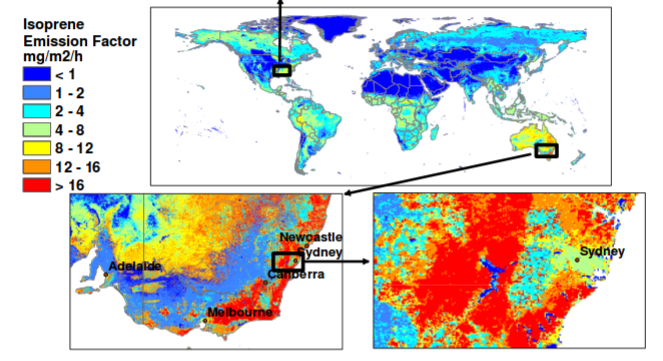
\includegraphics[width=\textwidth]{Figures/MeganIsoprene1_final.png}
      \caption{Global and Australian isoprene emission factors modified from \textcite{Guenther2006}.}
      \label{LR:Aus:fig_MEGAN_EF}
    \end{figure}
    
    
    Australia has a much greater diversity of tree species than is represented by MEGAN, however sparse measurements of emissions and BVOC concentrations makes model improvement difficult.
    %\textcite{Muller2008} show how isoprene (a key BVOC) is poorly captured by the MEGAN model and analyse the effect of changing the soil moisture parameter.
    %\textcite{Sindelarova2014} show reductions in modelled Australian isoprene emissions of 50\% when incorporating soil moisture in MEGAN estimates. 
    Uncertainties in isoprene emissions could explain why models of HCHO over Australia are poor at reproducing satellite measurements \parencite{Stavrakou2009}.
    
    
    % Australian BVOCs suffer even specifically from:
    Australia suffers from poor characterisation of plant emissions, partly because many of the emission factors are based on northern hemispheric data.
    Many plant emissions rates have not been published, such as those for any Australian acacias.
    Some Eucalypt emissions are based on samples from young trees, which may emit more isoprene than older trees \parencite{Emmerson2016}.
    Changes in parameterisation of soil moisture in the MEGAN model lead to large reductions ($38-58$\%) in Australian isoprene emission estimates, although errors remain \parencite{Sindelarova2014, Emmerson2019}.
    %Over Australia MEGAN suffers from a lack of studied plant functional types and their emissions \parencite[e.g.,][]{Muller2008}.
    %Emission rates from various species of Eucalyptus and other flora are highly complex, depending on current and recent weather, temperature, tree age, health, etc. \parencite{Guenther2012}. 
    
    
    % What did Emmerson do?
    The only VOC emission information currently available come from three campaigns: the Measurements of Urban, Marine and Biogenic Air (MUMBA), and the two Sydney Particulate Studies (SPS1 and SPS2) (see Section \ref{Model:datasets}).
    These measurements take place in south eastern Australia, and have suggested lower isoprene emissions than seen in models (by a factor of 2-6) \parencite{Emmerson2016}.
    %\textcite{Emmerson2016} %analyse EF sensitivity of a high resolution model of atmospheric chemistry over southeast Australia, comparing isoprene and monoterpene emissions against 4 separate campaigns.
    %analysed isoprene and monoterpene emissions sensitivities in a regional model of atmospheric chemistry over southeast Australia, using four campaigns that are also examined in this thesis.
    Several improvements are required as no simple scaling factor can completely fix the misrepresentation of isoprene emissions \parencite{Emmerson2016}.
    %\textcite{Emmerson2016} suggest that monoterpenes may be emitted in similar quantites to isoprene, with more measurements required to determine if this is so.
    %They compare emissions estimates from MEGAN against field campaign data and see overestimated isoprene emissions, as well as underestimated monoterpene emissions.
    %Their work suggests that MEGAN estimates of isoprene emissions may be 2-6 times too high, and monoterpene emissions $\sim3$ times too low over southeast Australia.
    % Brief overview of all the measurement campaigns.
    These measurements focus on air quality and biogenic VOCs and use several different instruments (including PTR-MS and GC-FID) to detect metrics such as air particulates, HCHO, isoprene, and meteorological information.
    Isoprene and many of its products can be difficult to measure accurately due to their short lifetimes, high reactivity, and optically thin natures.
    %An air-flight campaign (HIPPO) measuring over the Pacific ocean, with one flight passing along the NSW coastline, also provides isoprene and ozone concentrations in November 2009 \parencite{Wolfsy2011}.
    There is also an instrument at University of Wollongong (see Section \ref{Model:datasets:wollongong_ftir}) that provides 20 years of HCHO measurements, which is the only available long term HCHO vertical column measurement record in Australia comparable to satellite data. 
    Satellite HCHO column measurements can be limited by various factors including interfering species, water, clouds, orography, etc, and independent in-situ measurements are required to validate the data. % could cite john demol thesis for orography reference...? \parencite{Demol2010}.
    For further details on these campaigns and measurements, see Section \ref{Model:datasets}.
    
    % How could we improve this BVOC understanding?
    Improvements to emissions models require improved understanding of emissions from Australian vegetation and how they respond to meteorological and chemical parameters.
    However, constraining these processes is difficult given the lack of available isoprene measurements.
    Satellite measurements of HCHO can instead be used to estimate and improve Australian isoprene emissions without costly measurement campaigns.
    This is due to the near-linear relationship between HCHO and isoprene emissions \parencite[e.g.,][]{Palmer2001, Millet2006, Bauwens2016}.
    This method is explored in this thesis as described in Chapter \ref{BioIsop}.
  

  
\section{Aims}
\label{LR:Aims}

  \textbf{In this thesis I aim to improve understanding of natural contributions to ozone over Australia and the southern ocean.}
  The two largest contributors to tropospheric ozone concentrations are chemical production (driven by precursor emissions) and transport from the stratosphere.
  I aim to improve understanding of both of these sources using existing satellite and ground-based datasets along with modelled outputs from the GEOS-Chem chemical transport model.
  
  % Aim for Chapter 2: Modelling examination
  Estimation of BVOC emissions in Australia can be improved through satellite measurements of HCHO, one of isoprene's primary oxidation products.
  Satellites that overpass daily record %reflected solar (and emitted terrestrial) radiation, and give us 
  measurements over all of Australia.
  Combining satellite data with model outputs provides a platform for the understanding of natural processes, which are uncertain over Australia.
  Satellite measurements require modelled a priori vertical profiles of HCHO to estimate total column amounts.
  \textbf{I aim to recalculate satellite vertical columns of HCHO using updated model a priori information.}
  In this effort I aim to improve the understanding of the importance of relevant parameters (within GEOS-Chem) in calculating vertical columns of HCHO measured by satellite.
  This includes an examination of how well GEOS-Chem simulates several species such as NO$_x$, isoprene, and HCHO compared to both in-situ and remote measurement data that exists for Australia.
  Additionally, I detail the construction and effects of satellite data filters.
  The work towards this aim is detailed in Chapter \ref{Model}.
  %Soil moisture plays an important role in VOC emissions, as trees under stress may stop emitting various chemicals. 
  %This is especially true for Australia due to frequent droughts and wildfires.
  %The argument for improved understanding of land surface properties, specifically soil moisture, is an old one\parencite{Mintz1982, Rowntree1983, Chen2001}.
  
  % Aim for Chapter 3: Biogenic emissions estimation
  The technique of determining isoprene emissions from satellite detected HCHO is called satellite inversion.
  \textbf{I aim to determine isoprene emissions in Australia using a top-down inversion of satellite HCHO, through a modelled yield from isoprene to HCHO}.
  HCHO amounts and the yield of isoprene to HCHO over Australia is required to create top-down estimates.
  This process also requires careful examination of when the assumptions required within the inversion process are not valid.
  Due to the low availability of in-situ data over most of the Australian continent, a combination of modelled and satellite data can reduce the uncertainties of isoprene emissions from Australian landscapes.
  Improved emissions estimates will in turn improve the accuracy of CTMs, providing better predictions of atmospheric composition and its response to ongoing environmental change.
  The work towards fulfilling this aim is in Chapter \ref{BioIsop}.
  
  % Aim for Chapter 4: STT Ozone
  Stratospheric transport is the second largest driver of tropospheric ozone concentrations, and an improved understanding of transported ozone can be determined from ozonesonde measurements.
  \textbf{I aim to improve understanding of ozone transported to the troposphere from the stratosphere in Australia and the southern ocean.}
  Ozonesondes provide a glimpse of the vertical ozone profile up to $\sim 30$~km, and I use a Fourier filter to determine how often stratospheric transport is occurring at three sites: Melbourne, Macquarie Island, and Davis Station. 
  Transport event frequency analysis combined with modelled ozone distributions is used to derive a new method of detection and quantification of transported ozone as described in Chapter \ref{Ozone}.
  
  
  % Chapter 5: Conclusions?
  \textbf{Overall, I aim to describe relative importance of sources of tropospheric ozone in Australia, as well as their seasonality.}
  I will describe how modelled ozone is affected by updated isoprene emissions, comparing changes in GEOS-Chem outputs, and by ozone transport from the stratosphere..
  This thesis will provide new insight into tropospheric ozone in Australia.
  
